\documentclass{bookSolutions}

\title{Kreyszig  Introductory functional analysis with applications}
\author{Sergio Garrido}

\begin{document}
\maketitle

\tableofcontents

\section{Metric spaces}
\section{Metric space}


\begin{exercise}{1}
Show that the real line is a metric space.
\end{exercise}
\begin{proof}
We have that $d(x,y)=\absoluteValue{x-y}$ for $x,y,z\in\R$.

(M1): Certainly $d(x,y)$ is real valued, finite and nonnegative for all $x,y\in\R$.

(M2): We have $x=y$ if and only if $d(x,y)=\absoluteValue{x-y}=\absoluteValue{0}=0$.

(M3): Suppose, without loss of generality, that $x<y$. We have $d(x,y) =\absoluteValue{x-y} =-(x-y) =y-x$ and $d(y,x) =\absoluteValue{y-x} =y-x$, so that $d(x,y)=d(y,x)$.

(M4): We have $\absoluteValue{x-y} =\absoluteValue{(x-z)+(z-y)}\leq \absoluteValue{\absoluteValue{(x-z)}+\absoluteValue{(z-y)}} =\absoluteValue{(x-z)}+\absoluteValue{(z-y)}$. the inequality follows from the fact that $x-y \leq\absoluteValue{x-y}$ for all $x,y\in\R$, and the last equality follows from the fact that $\absoluteValue{(x-z)}, \absoluteValue{(z-y)}$ are both positive, so the absolute value of their sum is simply their sum.
\end{proof}

\begin{exercise}{2}
Does $d(x,y)=(x-y)^2$ define a metric on the set of all real numbers?
\end{exercise}
\begin{proof}
Although this metric candidate fulfills M1, M2 and M3, it doesn't fulfill M4. To see this, consider the points $x=1,y=2,z=1.5$. We have $d(x,y)=1$, $d(x,z)=0.25$ and $d(z,y)=0.25$, so that $1=d(x,y)\not\leq d(x,z)+d(z,y) =0.5$.
\end{proof}

\begin{exercise}{4}
Find all metrics on a set $X$ consisting of two points. Consisting of one point.
\end{exercise}
\begin{proof}
Let $d$ be the metric in both cases.

One point: Let $x\in X$. From M2, we must have that $d(x,x) =0$ so that the metric is the "zero" metric.

Two points: Let $x,y\in X$. From M1 we must have that $d$ is real valued, finite and nonnegative. Then $d(x,y)=c$ for some $c\in\R$ with $c>0$ and 0 otherwise.
\end{proof}

\begin{exercise}{5}
Let $d$ be a metric of $X$. Determine all constants $k$ such that (i) $kd$, (ii) $d+k$ is a metric on $X$
\end{exercise}
\begin{proof}
(i) Notice that if $k$ is 0 or negative it would violate M1. If $k>0$, then M1, M2 and M3 hold. To see M4 also holds, consider $x,y,z\in X$. Then we have that $d(x,y)\leq d(x,z)+d(z,y)$. Multiplying both sides of the inequality by $k$ we obtain $kd(x,y)\leq kd(x,z)+kd(z,y)$, as required.

(ii) If $k\neq 0$, then M2 doesn't hold because $d(x,x)+k=k$ but in a metric it should be 0. Hence we cannot add a real number to a metric.
\end{proof}

\begin{exercise}{6}
Show that $d$ in 1.1-6 satisfies the triangle inequality. Let $x=(x_1,x_2,\dots)$ be a bounded complex sequence, so that there exists a $c\in\R$ with $\absoluteValue{x_j}\leq c$ for all $j$. Let $x,y\in X$, and define $d(x,y)=\sup_{j\in\N}\absoluteValue{x_j-y_j}$.
\end{exercise}
\begin{proof}
We have $\absoluteValue{x_j-y_j} \leq \absoluteValue{x_j-z_j}+\absoluteValue{z_j-y_j}$. Since this holds for all $j$, we can take the supremum on both sides of the inequality to obtain $\sup_{j\in\N}\absoluteValue{x_j-y_j} \leq \sup_{j\in\N}(\absoluteValue{x_j-z_j}+\absoluteValue{z_j-y_j})$. Notice, however, that\\ $\absoluteValue{x_j-z_j}+\absoluteValue{z_j-y_j}\leq \sup_{j\in\N}\absoluteValue{x_j-z_j}+\sup_{j\in\N}\absoluteValue{z_j-y_j}$ for all $j$,\\ so that $\sup_{j\in\N}\absoluteValue{x_j-z_j}+\sup_{j\in\N}\absoluteValue{z_j-y_j}$ is an upper bound of $\absoluteValue{x_j-z_j}+\absoluteValue{z_j-y_j}$ and, by definition, greater than or equal to its supremum.
\end{proof}

\begin{exercise}{8}
Show that another metric $\tilde{d}$ on the set $X$ in 1.1-7 is defined by $\tilde{d}(f,g)=\int_a^b\absoluteValue{f(t)-g(t)}dt$.
\end{exercise}
\begin{proof}
Let $f,g,h\in C[a,b]$.

(M1): The integral of a nonnegative function ($\absoluteValue{f(x)-g(x)}$, in this case) is nonnegative. Integrals are real valued and because $f$ and $g$ are continuous, the image of a compact set (in this case $[a,b]$) is compact (Theorem 4.4.1. in Abbott's understanding analysis), so that the integral of $\absoluteValue{f(x)-g(x)}$ in $[a,b]$ is finite.

(M2): If $f=g$, clearly $d(f,g)=0$, on the other hand, if $\int_a^b\absoluteValue{f(x)-g(x)}dx =0$, it means that $f-g=0$. To see this, remember that $f-g$ is a continuous function, and that if there exists an $x\in [a,b]$ with $f(x)-g(x)>0$, then $f(x)-g(x)>0$ in an open interval around $x$ (see Carothers exercise 46), and then the integral would not be 0. Hence, $f=g$.

(M3): This follows from the symmetry of subtraction under absolute value.

(M4): We have 
\begin{align*}
    d(f,g) =& \int_a^b\absoluteValue{f(x)-g(x)}dx\\
    =&\int_a^b\absoluteValue{f(x)-h(x)+h(x)-g(x)}dx\\
    \leq& \int_a^b\absoluteValue{f(x)-h(x)}+\absoluteValue{h(x)-g(x)}dx\\
    =& \int_a^b\absoluteValue{f(x)-h(x)}dx+\int_a^b\absoluteValue{h(x)-g(x)}dx\\
    =& d(f,h) + d(h,g).
\end{align*}
\end{proof}

\begin{exercise}{9}
Show that $d$ in 1.1-8 is a metric. For any set $X$, and $x,y\in X$, we define $d(x,x)=0$ and $d(x,y)=1$ whenever $x\neq y$.
\end{exercise}
\begin{proof}
M1, M2 and M3 follow directly from the definition of the metric itself. To see that M4 holds, consider $x,y,z\in X$, then $1=d(x,y)\leq d(x,z)+d(z,y)=2$, as required.
\end{proof}

\begin{exercise}{11}
Prove (1): the generalized triangle inequality
\[
d(x_1,x_n)\leq d(x_1,x_2)+\dots+d(x_{n-1},x_n).
\]
\end{exercise}
\begin{proof}
We will prove this by induction.

Base case. If $n=3$, then $d(x_1,x_3)\leq d(x_1,x_2)+d(x_2,x_3)$.

Induction hypothesis. Suppose the inequality holds for $n-1$, so that\\ $d(x_1,x_{n-1})\leq d(x_1,x_2)+\dots+d(x_{n-2},x_{n-1})$.

Induction step. We have $d(x_1,x_n)\leq d(x_1,x_{n-1})+d(x_{n-1},x_n)\leq d(x_1,x_2)+\dots+d(x_{n-2},x_{n-1})+d(x_{n-1},x_n)$, as required.
\end{proof}

\begin{exercise}{12 (Triangle inequality)}
The triangle inequality has several useful consequences. For instance, using (1), show that $\absoluteValue{d(x,y)-d(z,w)}\leq d(x,z)+d(y,w)$
\end{exercise}
\begin{proof}
First, we have
\begin{align*}
    d(x,y) \leq d(x,z)+d(z,y) \leq d(x,z)+d(z,w)+d(y,z),
\end{align*}
so that $d(x,y)-d(z,w)\leq d(x,z)+d(y,w)$. On the other hand,
\begin{align*}
    d(z,w) \leq d(z,y)+d(y,w) \leq d(y,w)+d(z,x)+d(x,y),
\end{align*}
so that $-(d(y,w)+d(x,z))\leq d(x,y)-d(z,w)$. Putting these together we obtain the desired result.
\end{proof}

\begin{exercise}{13}
Using the triangle inequality show that $\absoluteValue{d(x,z)-d(y,z)}\leq d(x,y)$
\end{exercise}
\begin{proof}
We have $d(x,z)\leq d(x,y)+d(y,z)$, so that $d(x,z)-d(y,z)\leq d(x,y)$. On the other hand, $d(y,z)\leq d(x,y)+d(x,z)$, so that $-d(x,y)\leq d(x,z)-d(x,y)$. Combining these results together, we obtain that $\absoluteValue{d(x,z)-d(y,z)}\leq d(x,y)$.
\end{proof}

\begin{exercise}{15}
Show that nonnegativity of a metric follows from (M2) to (M4).
\end{exercise}
\begin{proof}
Let $x,y\in X$. We have $0=d(x,x)\leq d(x,y)+d(y,x)=2d(x,y)$, thus $0\leq d(x,y)$.
\end{proof}

\section{Further examples of metric spaces}


\begin{exercise}{3}
Show that the Cauchy-Schwarz inequality (11) implies 
\[
(\absoluteValue{x_1}+\dots+\absoluteValue{x_n})^2 
\leq n (\absoluteValue{x_1}^2+\dots+\absoluteValue{x_n}^2).
\]
\end{exercise}
\begin{proof}
Consider $(x_1,\dots,x_n)$ and $(1,\dots,1)$, $n$ times. Then the Cauchy-Schwarz inequality tells us
\[
\sum^n_{i=1}\absoluteValue{x_i} \leq
\sqrt{\sum_{i=1}^n\absoluteValue{x_i}^2}\sqrt{\sum_{i=1}^n\absoluteValue{1}^2} 
=\sqrt{\sum_{i=1}^n\absoluteValue{x_i}^2}\sqrt{n}.
\]
Squaring both sides of the inequality gives us the desired result.
\end{proof}

\begin{exercise}{4 (Space $l^p$)}
Find a sequence which converges to 0, but is not in any space $l^p$, where $1\leq p<+\infty$.
\end{exercise}
\begin{proof}
Consider the sequence $x^n=1/\log_2(n)$. This sequence converges to 0 because $\log_2(n)\to\infty$ as $n\to\infty$. However, we can do the Cauchy condensation test on the series $\sum_{n=1}^\infty 1/\absoluteValue{\log_2(n)}^p$ (to see whether $x^n$ is in $l^p$). We have 
\begin{align*}
    \sum_{n=1}^\infty \frac{2^n}{\absoluteValue{\log_2(2^n)}^p} 
    =\sum_{n=1}^\infty \frac{2^n}{\absoluteValue{n}^p}.
\end{align*}
Now using the ratio test on the sequence $2^n/\absoluteValue{n}^p$, we obtain
\[
\lim_{n\to\infty}\frac{2^{n+1}/\absoluteValue{(n+1)}^p}{2^n/\absoluteValue{n}^p} =2,
\]
so that the series does not converge for any $p$, giving us the desired result.
\end{proof}

\begin{exercise}{5}
Find a sequence which is in $l^p$ with $p>1$, but $x\notin l^1$.
\end{exercise}
\begin{proof}
We have that the series associated to the sequence $x^n=1/n$ does not converge for $p=1$ but it does for $p>1$, as required.
\end{proof}

\begin{exercise}{6 (Diameter, bounded set)}
The diameter $\delta(A)$ of a nonempty set $A$ in a metric space $(X,d)$ is defined to be 
\[
\delta(A) =\sup_{x,y\in A}d(x,y).
\]
$A$ is said to be bounded if $\delta(A)<\infty$. Show that $A\subseteq B$ implies $\delta(A)\leq\delta(B)$.
\end{exercise}
\begin{proof}
Since $\delta(B)=\sup{x,y\in B}d(x,y)$, then $\delta(B)$ is an upper bound for all the distances between the elements of $B$. However, because $A\subseteq B$, then the set of distances between the elements of $A$ is a subset of the set of distances between the elements of $B$. Hence $\delta(B)$ is also an upper bound for the set of distances between the elements of $A$. Thus, the least upper bound of such set, namely $\delta(A)$ is less than or equal to any other upper bound of such set, so that $\delta(A)\leq\delta(B)$, as required.
\end{proof}

\begin{exercise}{7}
Show that $\delta(A)=0$ (cf. exercise 6) if and only if $A$ consists of a single point.
\end{exercise}
\begin{proof}
Suppose $\delta(A)$ is 0, then for all $x,y\in A$, $d(x,y)=0$ (because $d$ is nonnegative), since $d(x,y)=0$ if and only if $x=y$, then $A$ consists of a single point. 

Conversely, suppose $A$ consists of a single point. Then $\delta(A) = \sup_{x,y\in A}d(x,y) =0$, as required.
\end{proof}

\begin{exercise}{11}
If $(X,d)$ is any metric space, show that another metric on $X$ is defined by
\[
\hat{d}(x,y)=\frac{d(x,y)}{1+d(x,y)},
\]
and $X$ is bounded in the metric $\hat{d}$.
\end{exercise}
\begin{proof}
M1, M2 and M3 follow directly from the properties of $d$ and the fact that the function $f(t)=t/(1+t)$ defined on the nonnegative reals does not alter these properties.

The proof that M4 holds for $\hat{d}$ is essentially the same as in 1.2-1, which I reproduce here for completeness. We have that $f'(t)=1/(1+t)^2$, which is positive, so that $f(t)$ is monotonically increasing. Thus, if $\absoluteValue{a+b}\leq \absoluteValue{a}+\absoluteValue{b}$, then $f(\absoluteValue{a+b})\leq f(\absoluteValue{a}+\absoluteValue{b})$. Knowing this, we have that 
\begin{align*}
    \frac{\absoluteValue{a+b}}{(1+\absoluteValue{a+b})} \leq& \frac{\absoluteValue{a}+\absoluteValue{b}}{1+\absoluteValue{a}+\absoluteValue{b}}\\
    \leq& \frac{\absoluteValue{a}}{1+\absoluteValue{a}} 
    + \frac{\absoluteValue{b}}{1++\absoluteValue{b}}.
\end{align*}
Replacing $a=d(x,z)$ and $b=d(z,y)$ in the above inequality we get the desired result.

To prove that $X$ is bounded under $\hat{d}$, consider the following two cases.

First: if $X$ is bounded under $d$, then $d(x,y)$ has an upper bound for all $x,y$ so that $\sup_{x,y\in X}\hat{d}(x,y)<\infty$.

Second: if $X$ is not bounded under $d$, then we have to check the limiting process of $\hat{d}$ whenever $d(x,y)\to\infty$ for some $x,y\in X$. In that case, we have $\lim_{d(x,y)\to\infty}\frac{d(x,y)}{1+d(x,y)}=1$, so that $\sup_{x,y\in X}\hat{d}(x,y)\leq \infty$, as required.
\end{proof}

\begin{exercise}{12}
Show that the union of two bounded sets $A$ and $B$ in a metric space is bounded. (Definition in exercise 6).
\end{exercise}
\begin{proof}
Suppose $A$ and $B$ are bounded. Let $a\in A\cup B$ be arbitrary and fix $a_0\in A$ and $b_0\in B$. If both $a_0,b_0$ are in either $A$ or $B$ then they they are bounded because both $A$ and $B$ are bounded. So suppose $a_0\in A$ and $b_0\in B$. By the generalised triangle inequality, with $x_1=a, x_2=a_0, x_3=b_0$ and $x_4=b$ (exercise 1.11), we obtain $d(a,b)\leq d(a,a_0)+d(a_0,b_0)+d(b_0,b)$. The first and the last terms of that inequality are bounded because $A$ and $B$ are bounded. Furthermore, by M1, $d(a_0,b_0)$ is finite. Thus, the right hand side of the inequality has an upper bound and since $a$ and $b$ were chosen arbitrarily, then $A\cup B$ is bounded.
\end{proof}

\begin{exercise}{13 (Product of metric spaces)}
The Cartesian product $X=X_1\times X_2$ of two metric spaces $(X_1, d_1)$ and $(X_2, d_2)$ can be made into a metric space $(X, d)$ in many ways. For instance, show that a metric $d$ is defined by $d(x,y)=d_1(x_1,y_1)+d_2(x_2,y_2)$, where $x=(x_1,x_2)$ and $y=(y_1,y_2)$.
\end{exercise}
\begin{proof}
M1, M2 and M3 follow from the fact that $d$ is an addition and the properties of $d_1$ and $d_2$. To see that M4 holds, let $x,y,z\in X_1\times X_2$. We have $d(x,y) =d_1(x_1,y_1)+d_2(x_2,y_2) \leq d_1(x_1,z_1)+d_1(z_1,y_1) + d_2(x_2,z_2)+d_2(z_2,y_2) = d(x,z)+d(z,y)$, as required.
\end{proof}

\begin{exercise}{14}
Show that another metric on $X_1\times X_2$ (as in exercise 13) is defined by $\hat{d}(x,y)=\sqrt{d_1(x_1,y_1)^2+d_2(x_2,y_2)^2}$.
\end{exercise}
\begin{proof}
M1, M2 and M3 follow directly from the properties of $d_1$ and $d_2$ and the functions that compose them: first squaring, then addition and then taking root, all of which preserve these properties of metrics. To see M4 holds, let $x,y,z\in X_1\times X_2$. We have 
\begin{align*}
    \hat{d}(x,y) =& [d_1(x_1,y_1)^2+d_2(x_2,y_2)^2]^{1/2}\\
    \leq& [[d_1(x_1,z_1)+d_1(z_1,y_1)]^2+[d_2(x_2,z_2)+d_2(z_2,y_2)]^2]^{1/2}\\
    =& [d_1(x_1,z_1)^2+2d_1(x_1,z_1)d_1(z_1,y_1)+d_1(z_1,y_1)^2\\
    &+ d_2(x_2,z_2)^2+2d_2(x_2,z_2)d_2(z_2,y_2)+d_2(z_2,y_2)^2]^{1/2}
\end{align*}
squaring both sides of the inequality, and using the the Cauchy-Schwarz inequality in those terms that contain a factor of 2:
\begin{align*}
    \hat{d}(x,y)^2 
    \leq&  d_1(x_1,z_1)^2+d_2(x_2,z_2)^2 +d_1(z_1,y_1)^2+d_2(z_2,y_2)^2\\
    &+2\sqrt{\sum_{i=1}^2d_i(x_i,z_i)^2}\sqrt{\sum_{i=1}^2d_i(z_i,y_i)^2}\\
    =& \hat{d}(x,z)^2 + \hat{d}(z,y)^2+ 2(\hat{d}(x,z)\hat{d}(z,y))\\
    =& (\hat{d}(x,z)+\hat{d}(z,y))^2.
\end{align*}
Taking square root on both sides of the inequality gives us the desired result.
\end{proof}

\begin{exercise}{15}
Show that a third metric on $X_1\times X_2$ (as in exercise 13) is defined by $\bar{d}(x,y)=\max[d_1(x_1,y_1),d_2(x_2,y_2)]$. (The metrics in exercises 13 to 15 are of practical importance, and other metrics on $X$ are possible).
\end{exercise}
\begin{proof}
M1, M2 and M3 follow directly from the properties of $d_1$ and $d_2$ and the fact that $\max$ does not affect these properties. To see M4 also holds, let $x,y,z\in X_1\times X_2$. We have
\begin{align*}
    \bar{d}(x,y) 
    =& \max[d_1(x_1,y_1),d_2(x_2,y_2)]\\
    \leq& \max[d_1(x_1,z_1)+d_1(z_1,y_1),d_2(x_2,z_2)+d_2(z_2,y_2)]\\
    \leq& \max[d_1(x_1,z_1),d_2(x_2,z_2)]
    + \max[d_1(z_1,y_1), d_2(z_2,y_2)]\\
    =& \bar{d}(x,z)+\bar{d}(z,y),
\end{align*}
where the last inequality follows from the fact that we are splitting the sums on the second line by choosing the greatest element of each sum and adding them together, hence the sum of the $\max$ is greater than the $\max$ of the sums.
\end{proof}
\section{Open set, closed set, neighborhood}


\begin{exercise}{1}
Justify the terms ``open ball'' and ``closed ball'' by proving that (a) any open ball is an open set, (b) any closed ball is a closed set.
\end{exercise}
\begin{proof}
(a) This follows the same logic as in the converse of exercise 4.

(b) Consider the closed ball with radius $r$ around $x$, $B=B(x;r)$. Let $y\in B^C$, and $r'=\min[d(y,x+r), d(y,x-r)]$, we have that $B(y;r'/2)\subseteq B^C$, so that for any point in $B^C$ there is an open ball containing it, that is, $B^C$ is open and thus $B$ is closed.
\end{proof}

\begin{exercise}{2}
What is an open ball $B(x_0; 1)$ on $\R$? In $\C$ (Cf. 1.1-5)?  In $C[a,b]$ (Cf. 1.1-7)? Explain the following figure.
\begin{figure}[H]
    \centering
    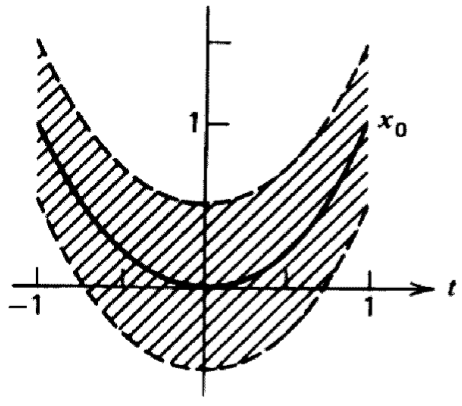
\includegraphics[width=0.5\textwidth]{kreyszig/assets/sec1-3-ex2.png}
    \caption{Region containing the graphs of all $x\in C[-1,1]$ which constitute the $\epsilon$-neighborhood, with $\epsilon=1/2$, of $x_0\in C[-1,1]$ given by $x_0(t)=t^2$.}
    \label{fig:fig1-3}
\end{figure}
\end{exercise}
\begin{proof}
$\R$: An open interval of the form $(a,b)$, where $b-a=2$ and the midpoint is $x_0$.

$\C$: If we think of $\C$ as $\R^2$ then it is a circle centered at $x_0$ with radius $1$, without the circumference of the circle.

$C[a,b]$: All the functions $g$ so that $\absoluteValue{g(t)-x_0(t)}<1$ for all $t$. 

We can see something similar in \Cref{fig:fig1-3}, where the shaded area is the area where the functions with $\absoluteValue{g(t)-t^2}<1/2$ can go through, for $t\in[-1,1]$.
\end{proof}

\begin{exercise}{3}
Consider $C[0,2\pi]$ and determine the smallest $r$ such that $g\in \hat{B}(f;r)$, where $f(t)=\sin t$ and $g(t)=\cos t$.
\end{exercise}
\begin{proof}
$r=1$ suffices, since the largest difference between $\sin t$ and $\cos t$ is 1 whenever $t=0$.
\end{proof}

\begin{exercise}{4}
Show that any nonempty set $A\subseteq (X,d)$ is open if and only if it is a union of open balls.
\end{exercise}
\begin{proof}
($\Rightarrow$) Suppose $A$ is open, then for every point in $x$ there is an open ball which is a subset of $A$. Thus $A$ is composed of open balls. That is, $A$ is a union of open balls.

($\Leftarrow$) Suppose $A$ is a union of open balls. Then any point in $x\in A$ belongs to one of these open balls, say $B(y;r)$. Let $r'=\min[d(x,y+r), d(x,y-r)]$, then $B(x;r')\subseteq B(y;r)\subseteq A$, so that there is an open ball around $x$ and $A$ is open.
\end{proof}

\begin{exercise}{5}
It is important to realise that certain sets may be open and closed at the same time. (a) Show that this is always the case for $X$ and $\emptyset$. (b) Show that in a discrete metric space $X$ (Cf. 1.1-8), every subset is open and closed.
\end{exercise}
\begin{proof}
(a) On page 19 Kreyszig proved that $\emptyset$ and $X$ are open. A set is closed if its complement is open. Hence given $X^C=\emptyset$ and $\emptyset^C=X$, both $X$ and $\emptyset$ are closed.

(b) From (a) we know that $X$ and $\emptyset$ are open and closed so let's consider a non trivial subset of $X$. Notice that every nonempty subset of $X$ is open, because for any $x\in X$, the set $\set{x}$ is a ball $B(x; r)$ for any $r<1$. But this means that the complement of any nonempty subset of $X$ is open because the same holds for any element of $X$. Hence, all subsets of $X$ are open and closed (clopen).
\end{proof}

\begin{exercise}{7}
Describe the closure of each of the following subsets. (a) The integers on $\R$, (b) the rational numbers on $\R$, (c) the complex numbers with rational real and imaginary parts in $\C$, (d) the disk $\set{z: \absoluteValue{z}<1}\subseteq\C$.
\end{exercise}
\begin{proof}
(a) Let $x\in\R$ and $x\notin\Z$. Notice that there are two integers $a,b$ so that $a<x<b$. Let $r=\min[x-a, b-x]$. We then have that $B(x,r)$ does not contain any element of $\Z$ and thus $x$ is not an accumulation point of $\Z$ in $\R$. As a result, $\Z=\overline{\Z}$ in $\R$.

(b) By the density of the rationals in the reals, any open ball around a rational contains an irrational number and hence it is an accumulation point. As a result, $\overline{\Q}=\R$.

(c) Following the same logic of (b), the closure of the complex numbers with rational real and imaginary parts is $\C$.

(d) This is similar to (b) and (c). Simply let $x\in\C$ have $\absoluteValue{x}=1$. For any $\epsilon>0$ we will always find that the ball $B(x;\epsilon)$ will contain an element of $\set{z: \absoluteValue{z}<1}$, so that $x\in\overline{\set{z: \absoluteValue{z}<1}}$. On the other hand, any number $y\in\C$ with $\absoluteValue{y}>1$ has an $\epsilon$-neighborhood so that no element of $\set{z: \absoluteValue{z}<1}$ belongs to it. Putting this together, we conclude that $\overline{\set{z: \absoluteValue{z}<1}}=\set{z: \absoluteValue{z}\leq 1}$.
\end{proof}

\begin{exercise}{8}
Show that the closure $\overline{B(x_0;r)}$ of an open ball $B(x_0;r)$ in a metric space can differ from the closed ball $\hat{B}(x_0;r)$.
\end{exercise}
\begin{proof}
Consider a set $X$ with the discrete metric. We have that $\hat{B}(x,1)=X$ for any $x\in X$. However, let $x,y\in X$ and consider the open ball $B(x;1)=\set{x}$. Think of the $\epsilon$-neighborhood around $y$ with $\epsilon=1/2$. Such $\epsilon$-neighborhood does not contain any element of $B(x;1)$, and so $y$ is not an accumulation point of $B(x;1)$. As a result, $B(x;1)=\overline{B(x;1)}\neq\hat{B}(x,1)=X$, as required.
\end{proof}

\begin{exercise}{9}
Show that 
\begin{enumerate}
    \item $A\subseteq\overline{A}$.
    \item $\overline{\overline{A}}=\overline{A}$.
    \item $\overline{A\cup B}=\overline{A}\cup\overline{B}$.
    \item $\overline{A\cap B}\subseteq\overline{A}\cap\overline{B}$.
\end{enumerate}
\end{exercise}
\begin{proof}
\begin{enumerate}
    \item By definition $\overline{A}$ contains $A$.
    \item We will prove this by double containment. $\overline{\overline{A}}\supseteq\overline{A}$ follows directly from the definition of closure. For the other direction, let $x\in \overline{\overline{A}}$. Then $x$ is either:
    
    (i) In $\overline{A}$, in which case $x\in\overline{\overline{A}}$ or,
    
    (ii) $x$ is an accumulation point of $\overline{A}$ not in $\overline{A}$.
    
    So suppose $x\notin \overline{A}$. Fix $\epsilon>0$, because $x$ is an accumulation point, there exists $y\in\overline{A}$ such that $d(x,y)\leq \epsilon/2$, and likewise because $y$ is in $A$ or it is one of its accumulation points, then  there exists $z\in A$ such that $d(y,z)\leq \epsilon/2$. Hence, $d(x,z)\leq d(x,y)+d(y,z) =\epsilon$ and so $x$ is an accumulation point of $A$ resulting in $x\in\overline{A}$. This contradicts (ii) so it must be the case that $x\in\overline{\overline{A}}$.
    \item We will prove this by double containment. 

    ($\subseteq$) Let $x\in\overline{A}\cup\overline{B}$. Then $x$ is either in $A$ or $B$ or an accumulation of either. If $x\in A$ or $x\in B$, then $x\in\overline{A}\cup\overline{B}$, so suppose $x\notin A,B$. Without loss of generality, suppose $x$ is an accumulation point of $A$. Then for every $\epsilon>0$, an open ball centered around $x$ with radius $\epsilon$ contains an element of $A$. But certainly it contains an element of $A\cup B$, so that $x\in\overline{A\cup B}$.

    ($\supseteq$) Let $x\in\overline{A\cup B}$. Then either $x\in A\cup B$ or $x$ is an accumulation of the union. In the former case, we would have that $x\in\overline{A}$ or $x\in\overline{B}$, so suppose that's not the case. Since $x$ is an accumulation point of $A\cup B$, then it must be the case there are infinite elements of $A\cup B$ that intersect open balls centered at $x$ (suppose this wasn't the case, then we could take the minimum of the distances between $x$ and every one of those elements of $A\cup B$, and then the open ball centered at $x$ with half such distance would not contain any element of $A\cup B$). However, this implies that there are either infinite elements of $A$ or infinite elements of $B$ that intersect open balls centered around $x$ (of any arbitrarily small radius), so that either $x\in\overline{A}$ or $x\in\overline{B}$.
    \item Suppose $x\in\overline{A\cap B}$, then either $x\in A\cap B$ or $x$ is an accumulation point of such set. If $x\in A\cap B$, then $x\in A$ and $x\in B$ so certainly $x\in\overline{A}\cap\overline{B}$ since $A\subseteq\overline{A}$ and $B\subseteq\overline{B}$. So suppose $x$ is an accumulation point of $A\cap B$. This implies that for every $\epsilon>0$, the open ball of radius $\epsilon$ centered at $x$ contains an element $y\in A\cap B$. Thus, for every $\epsilon>0$, there exists an element of $A$ such that it belongs to the open ball centered around $x$, so that $x\in\overline{A}$, following the same argument we can conclude that $x\in\overline{B}$ as well. That is, $x\in\overline{A}\cap\overline{B}$.
    \end{enumerate}
\end{proof}

\begin{exercise}{11 (Boundary)}
A boundary point $x$ of a set $A\subseteq (X,d)$ is a point of $X$ (which may or may not belong to $A$) such that every neighborhood of $x$ contains points of $A$ as well as points not belonging to $A$; and the boundary (or frontier) of $A$ is the set of all boundary points of $A$. Describe the boundary of (a) the intervals $(-1,1), [-1,1), [-1,1]$ on $\R$; (b) the set of all rational numbers on $\R$; (c) the disks $\set{z:\absoluteValue{z}<1}\subseteq\C$ and $\set{z:\absoluteValue{z}\leq 1}\subseteq\C$.
\end{exercise}
\begin{proof}
(a) For all intervals $-1$ and 1 are the boundary points. Simply consider for any $\epsilon>0$ the open ball around any of these two points. We will obtain than points in the intervals (and outside of them), are in such ball.

(b) Since the rationals are dense in $\R$, any open ball around any rational will contain both rationals and irrationals. Furthermore, for any irrational, we can find a rational that gets arbitrarily close to it. Hence, $\R$ is the boundary of $\R$.

(c) In both cases, the set $\set{z:\absoluteValue{z}=1}\subseteq\C$ is the boundary of the disks. That is because for any open ball around these points, we can find elements withing the disks and outside of them.
\end{proof}

\begin{exercise}{12 (Space $B[a,b]$)}
 Show that $B[a,b]$, $a<b$ is not separable (Cf. 1.2-2).
\end{exercise}
\begin{proof}
Suppose, for the sake of contradiction, that $B[a,b]$ is separable. Then there exists a countable set, call it $\cF$, of functions so that for all functions in $g\in B[a,b]$, either $g\in\cF$, or for all $\epsilon>0$, there exists a function $f\in\cF$ with $f\in B(g;\epsilon)$.

Since $\cF$ is countable we can find a bijection between $\cF$ and $\N$, so that we can have a sequence of distinct numbers, $(x_n)$ where each $x_i\in[a,b]$ and $x_n$ can be mapped to a function, say $f_n\in\cF$. Now let $h\in B[a,b]$ be defined as follows: for $h(x_n)=f_n(x_n)+1$ and 0 otherwise. We have that the open ball $B(h;1/2)$ does not contain any element of $\cF$, so that $h$ is not an accumulation point of $\cF$. Thus, $\overline{\cF}\neq B[a,b]$ and $B[a,b]$ is not separable. 
\end{proof}

\begin{exercise}{13}
Show that a metric space $X$ is separable if and only if $X$ has a countable subset $Y$ with the following property. For every $\epsilon>0$ and every $x\in X$ there is a $y\in Y$ such that $d(x,y)<\epsilon$.
\end{exercise}
\begin{proof}
($\Rightarrow$) Suppose $X$ is separable. Then there exists a countable subset $Y\subseteq X$ so that $\overline{Y}=X$. But this means that for every $x\in X$, either $x\in Y$ or that for all $\epsilon>0$, there exists a $y\in Y$ with $y\in B(x, \epsilon)=\set{z\in X:d(x,z)<\epsilon}$, giving us the desired result.

($\Leftarrow$) Suppose there exists a countable subset $Y\subseteq X$ so that for every $\epsilon>0$, and every $x\in X$, there exists a $y\in Y$ with $d(x,y)<\epsilon$. Then this means that every $x\in X$ is an accumulation point, because for every $x$ and $\epsilon>0$ we can find $y\in Y$ with $y\in B(x,\epsilon)$. However, since all $x\in X$ are accumulation points of $Y$, then $\overline{Y}=X$, giving us that $X$ is separable, as required.
\end{proof}

\begin{exercise}{14 (Continuous mapping)} Show that a mapping $T:X\to Y$ is continuous if and only if the inverse image of any closed set $M\subseteq Y$ is a closed set in $X$.
\end{exercise}
\begin{proof}
Let $M$ be closed so that $M^C$ is open. By definition, we have that $(T^{-1}(M))^C=\set{x\in X:T(x)\notin M}=T^{-1}(M^C)$. 

For the ($\Rightarrow$) proof, if $T$ is continuous, then the inverse image of an open set is open, so that $T^{-1}(M^C)$ is open and by the equality above, then the inverse image of a closed set is closed. That is, $(T^{-1}(M))^C$ is open. 

For the converse, $(\Leftarrow)$, if the inverse image of a closed set is closed, so that $(T^{-1}(M))^C$ is open, by the equality above, we get that $T^{-1}(M^C)$ is open, so that the inverse image of an open set is open. That is, $T$ is continuous.
\end{proof}

\begin{exercise}{15}
Show that the image of an open set under a continuous mapping need not be open.
\end{exercise}
\begin{proof}
We have that $f:\R\to\R$ given by $f(x)=x^2$ is continuous. Consider the open set $A=(-1,1)\in\R$. We have that $f(A)=[0,1)$, which is not open in $\R$ because there is no open ball around 0 fully contained in $[0,1)$.
\end{proof}

\subsection{Convergence, Cauchy sequence, completeness}

\begin{exercise}{1 (Subsequence)}
If a sequence $(x^n)$ in a metric space $X$ is convergent and has limit $x$, show that every subsequence $(x^{n_k})$ of $(x^n)$ is convergent and has the same limit $x$.
\end{exercise}
\begin{proof}
Let $(x_{n_k})$ be a subsequence of $(x^n)$. Since $(x^n)$ converges to $x$, then for all $\epsilon>0$, there exists an $N\in\N$ so that for all $n>N$, it holds that $d(x^n,x)<\epsilon$. Fix $\epsilon>0$, and find $N\in\N$ as above. Now $N<n_K$ for some $K\in\N$, so that for all $k>K$ (and thus $n_k>N$, it holds that $d(x^{n_k},x)<\epsilon$ and $(x^{n_k})\to x$, as desired.
\end{proof}

\begin{exercise}{2}
If $(x^n)$ is Cauchy and has a convergent subsequence, say, $x^{n_k}\to x$, show that $(x^n)$ is convergent with the limit $x$.
\end{exercise}
\begin{proof}
Because $(x^n)$ is Cauchy, then for all $\epsilon>0$, there exists an $N\in\N$, so that for all $n,m>N$, it holds that $d(x^n,x^m)<\epsilon/2$. Likewise, there exists an $K\in\N$, so that for all $k>K$, it holds that $d(x^{n_K},x)<\epsilon/2$. Let $N'=\max[N,n_K]$, then for $n>N'$ and a fixed $n_k>N'$, we have $d(x^n,x)\leq d(x^n,x^{n_k})+d(x^{n_k},x)<\epsilon$
\end{proof}

\begin{exercise}{3}
Show that $x^n\to x$ if and only if for every neighborhood $V$ of $x$ there is an integer $n_0$ such that $x^n\in V$ for all $n>n_0$.
\end{exercise}
\begin{proof}
($\Rightarrow$) Suppose $x^n\to x$. Then for every $\epsilon>0$ there exists an $N$ so that for all $n>N$, it holds that $d(x^n,x)<\epsilon$. That is, no matter the size of the $\epsilon$-neighborhood inside $V$, we can find such $n_0$.

($\Leftarrow$) Suppose that for every neighborhood of $x$ we can find an $n_0$ so that for $n>n_0$ it holds that $x^n\in V$. Fix $\epsilon>0$ and let $V=B(x;\epsilon)$, then for $n>n_0$, it holds that $d(x^n,x)<\epsilon$. That is $x^n\to x$.
\end{proof}

\begin{exercise}{4 (Boundedness)}
Show that a Cauchy sequence is bounded.
\end{exercise}
\begin{proof}
A sequence is Cauchy if for all $\epsilon>0$, there exists an $N\in\N$ so that for all $n,m\geq N$, it holds that $d(x^n,x^m)<\epsilon$. Let $\delta=\max\set{d(x^n,x^k):k<N}$. We have that $\delta+\epsilon$ is a bound for the sequence because for arbitrary $x^n$ and $x^m$ in the sequence, $d(x^n,x^m)<\delta$ if $n,m<N$, $d(x^n,x^m)<\epsilon$ if $n,m\geq N$, and $d(x^n,x^m)\leq d(x^n,x^N)+d(x^N,x^m)=\delta+\epsilon$, if $n<N$ and $m\geq N$. 
\end{proof}

\begin{exercise}{5}
Is boundedness of a sequence in a metric space sufficient for the sequence to be Cauchy? Convergent?
\end{exercise}
\begin{proof}
Unfortunately no. Consider the real sequence (under the usual metric) given by $x^n=1$ if $n$ is even and $x^n=0$ if $n$ is odd. This sequence is pointwise bounded but certainly not Cauchy, nor convergent.
\end{proof}

\begin{exercise}{6}
If $(x^n)$ and $(y_n)$ are Cauchy sequences in a metric space $(X,d)$, show that $(a^n)$, where $a_n=d(x^n,y^n)$, converges. Give illustrative examples.
\end{exercise}
\begin{proof}
From exercise 1.1.12, we know that $\absoluteValue{d(x,y)-d(z,w)}\leq d(x,z)+d(y,w)$, so that $\absoluteValue{d(x^n,y_n)-d(x^m,y^m)}\leq d(x^n,x^m)+d(y^n,y^m)$. Fix $\epsilon>0$, since $(x^n)$ and $(y^n)$ are Cauchy, there exist $N,N'\in\N$, so that for all $n,m>N$ and $n',m'>N'$, it holds that $d(x^n,x^m)<\epsilon/2$ and $d(y^{n'},y^{m'})<\epsilon/2$. Let $M=\max[N,N']$, and $n,m>M$. We have $\absoluteValue{d(x^n,y^n)-d(x^m,y^m)}\leq d(x^n,x^m)+d(y^n,y^m)<\epsilon$, so that $(a^n)$ is Cauchy. Since $(a^n)$ is a Cauchy sequence in the reals, by the completeness of the reals (1.4-4), $(a^n)$ converges, as required.
\end{proof}

\begin{exercise}{8}
If $d_1$ and $d_2$ are metrics on the same set $X$ and there are positive numbers $a$ and $b$ such that for all $x,y\in X$, $ad_1(x,y)\leq d_2(x,y)\leq bd_1(x,y)$, show that the Cauchy sequences in $(X,d_1)$ and $(X,d_2)$ are the same.
\end{exercise}
\begin{proof}
Let $(x^n)$ be Cauchy in $(X,d_2)$. For $\epsilon>0$ there exists an $N\in\N$ such that for all $n,m>N$, it holds that $d_2(x^n,x^m)<\epsilon/a$, hence $d_1(x^n,x^m)<ad_2(x^n,x^m)<a\epsilon/a=\epsilon$ and $(x^n)$ is also Cauchy in $(X,d_1)$. We can prove that a Cauchy sequence in $(X,d_1)$ is Cauchy in $(X,d_2)$ mutatis mutandis.
\end{proof}

\begin{exercise}{9}
Using exercise 8, show that the metric space in exercises 13 to 15 of Section 1.2 have the same Cauchy sequences.
\end{exercise}
\begin{proof}
We have that 
\[
\max[d_1(x_1,y_1),d_2(x_2,y_2)]
\leq d_1(x_1,y_1)+d_2(x_2,y_2)
\leq 2\max[d_1(x_1,y_1),d_2(x_2,y_2)],
\]
so that $\bar{d}(x,y)$ and $d(x,y)$ are equivalent.

Furthermore,
\[
\max[d_1(x_1,y_1),d_2(x_2,y_2)]
\leq \sqrt{d_1(x_1,y_1)^2+d_2(x_2,y_2)^2}
\leq \sqrt{2}\max[d_1(x_1,y_1),d_2(x_2,y_2)],
\]
so that $\bar{d}(x,y)$ and $\hat{d}(x,y)$ are equivalent.

Since being equivalent in this sense is an equivalence relation, then $d(x,y)$ and $\hat{d}(x,y)$ are equivalent, as required.
\end{proof}

\begin{exercise}{10}
Using the completeness of $\R$, prove the completeness of $\C$.
\end{exercise}
\begin{proof}
Let $(x^n)$ be a Cauchy sequence in $\C$. That is, $x^n$ can be written as $a^n+ib^n$ for $a^n,b^n\in\R$. Let $\epsilon>0$, then we can find $N\in\N$ so that for any $n,m>N$, we have that $d(x^n,x^m)=\sqrt{(a^n-a^m)^2+(b^n-b^m)^2}<\epsilon$. 

From the previous statement, we can see that for the same $n$ and $m$, it holds that $d(a^n,a^m)\leq \epsilon$ and $d(b^n,b^m)\leq \epsilon$ under the euclidean metric. That is, $(a^n)$ and $(b^n)$ are Cauchy. Since they are Cauchy, they converge to say $a$ and $b$ so that $x^n$ converges to $a+ib$, as required.
\end{proof}
\subsection{Examples. Completeness proofs}


\begin{exercise}{1}
Let $a,b\in\R$ and $a<b$. Show that the open interval $(a,b)$ is an incomplete subspace of $\R$, whereas the closed interval $[a,b]$ is complete.
\end{exercise}
\begin{proof}
By section 1-4, we know that $\R$ is a complete metric space. By Theorem 1.4-7, we know that a subspace, $M$, of a complete metric space, $X$, is complete if and only if $M$ is closed in $X$. We have that $(a,b)$ is not closed in $\R$, because $a$ and $b$ don't belong to the set but they are limit points of the set. Hence $(a,b)$ is not complete. On the other hand, $[a,b]$ is closed in $\R$ and thus a complete subspace of $\R$.
\end{proof}

\begin{exercise}{2}
Let $X$ be the space of all ordered $k$-tuples $x=(x_1,x_2,\dots,x_k)$ of real numbers and $d(x,y)=\max_j\absoluteValue{x_j-y_j}$ where $y=(y_1,\dots,y_k)$. Show that $(X,d)$ is complete.
\end{exercise}
\begin{proof}
We will follow a similar strategy as in the text. Let $x^{(n)}$ be a Cauchy sequence in the defined space. Then for $\epsilon>0$, there exists an $N\in\N$ so that for all $n,m>N$, it holds that $d(x^n,x^m)=\max_j\absoluteValue{x^n_j-x^m_j}<\epsilon$. This means that for all $j$, we have that $\absoluteValue{x^n_j-x^m_j}<\epsilon$. But this implies that for each $j$, the sequence $(x^n)$ in $\R$ is Cauchy and by the completeness of $\R$, it converges. Now let $x=(x_1,\dots,x_k)$, for a given $\epsilon>0$, we can find $N\in\N$ with $d(x^n,x)=\max_j\absoluteValue{x^n_j-x_j}<\epsilon$, so that $x^n\to x$, as required. 
\end{proof}

\begin{exercise}{3}
Let $M\subseteq l^\infty$ be the subspace consisting of all sequences with at most finitely many nonzero terms. Find a Cauchy sequence in $M$ which does not converge in $M$, so that $M$ is not complete.
\end{exercise}
\begin{proof}
First let's define a target sequence not in $M$: $x=(1,1/2,1/3,\dots)$. Now consider the sequence of sequences given by $x^1=(1,0,0,\dots),\,x^2=(1,1/2,0,\dots),\,x^3=(1,1/2,1/3,\dots)$. To see that $x^n\to x$, notice that $d(x^n,x)=\sup_{j\in\N}\absoluteValue{x^n_j-x_j}=1/n$. Then, after fixing $\epsilon>0$, we can choose $N\in\N$ so that for all $n>N$, $1/n<\epsilon$. Then we have $d(x^n,x)<1/n<\epsilon$, as required. However all elements of $x$ are nonzero so $l^\infty$ is not complete.
\end{proof}

\begin{exercise}{5}
Show that the set $X$ of all integers with metric $d$ defined by $d(m,n)=\absoluteValue{m-n}$ is a complete metric space.
\end{exercise}
\begin{proof}
We can prove this using Theorem 1.4-7. $\Z$ with the usual metric on $\R$ is a subspace of $\R$. We have that $\Z$  is closed in $\R$, because its complement is open (it is a union of open intervals). Hence, Theorem 1.4-7 tells us that $\Z$ is complete.
\end{proof}

\begin{exercise}{6}
Show that the set of all real numbers constitutes an incomplete metric space if we choose $d(x,y)=\absoluteValue{\arctan x-\arctan y}$.
\end{exercise}
\begin{proof}
Consider the sequence given by $x^n=\tan(\pi/2-1/n)$, then under the defined metric, the sequence is Cauchy (because $d(x^m,x^n)=\absoluteValue{1/m-1/n}$, so for a fixed $\epsilon>0$, we can choose an $N\in\N$ so that for all $n,m>N$, it holds that $d(x^n,x^m)<\epsilon$. However, since $\tan(\pi/2)$ is not defined, then the limit is not in $\R$, and hence $\R$ is not complete under this metric.
\end{proof}

\begin{exercise}{8 (Space $C[a,b]$)}
Show that the subspace $Y\subseteq C[a,b]$ consisting of all $x\in C[a,b]$ such that $x(a)=x(b)$ is complete
\end{exercise}
\begin{proof}
We will prove the statement using Theorem 1.4-7 which asserts that a subset of a complete space is itself complete if it is closed. To do that, we need to prove $Y^C$ is open. Let $f\in Y^C$ and choose $\epsilon$ such that $\absoluteValue{f(a)-f(b)}>\epsilon>0$. Now consider the open ball $B(f;\epsilon/2)$. For any $g\in B(f;\epsilon/2)$, we have that 
\begin{align*}
    &\absoluteValue{g(b)-g(a)+f(a)-f(a)+f(b)-f(b)} \\
    >& \absoluteValue{f(b)-f(a)} -\absoluteValue{g(b)-f(b)} -\absoluteValue{g(a)-f(a)}\\
    >& \epsilon-\absoluteValue{g(b)-f(b)}-\absoluteValue{f(a)-g(a)}>0
\end{align*}
 The last inequality being true because $\absoluteValue{g(b)-f(b)}-\absoluteValue{f(a)-g(a)}<\epsilon$. Thus, $g\notin Y$ so that $Y^C$ is open, $Y$ is closed, and by 1.4-7, complete.
\end{proof}

\begin{exercise}{10 (Discrete metric)}
Show that a discrete metric space (cf. 1.1-8) is complete.
\end{exercise}
\begin{proof}
Let $(x^n)$ be a Cauchy sequence in a discrete space. Then it must be the case that for $N\in\N$, $x^n$ is the same for all $n>N$, otherwise $\epsilon<1$ would be enough to break the Cauchy criterion. But since this element must be in the space itself, then we can choose it as the limit of the sequence, and hence the discrete space is complete.
\end{proof}

\begin{exercise}{11 (Space $s$)}
Show that in the space $s$ (cf. 1.2-1) we have $x^n\to x$ if and only if $x^n_j\to x_j$ for all $j=1,2,\dots$, where $x^n=(x^n_1, x^n_2,\dots)$ and $x=(x_1, x_2,\dots)$.
\end{exercise}
\begin{proof}
For reference, recall that $s$ is the set of all sequences of complex numbers and the following metric:
\[
d(x,y)=\sum_{j=1}^\infty \frac{1}{2^j}\frac{\absoluteValue{x_j-y_j}}{1+\absoluteValue{x_j-y_j}}.
\]

($\Rightarrow$) Suppose $x^n\to x$. Then for $1>\epsilon>0$, there exists an $N\in\N$, so that for all $n>N$, it holds that
\[
d(x^n,x)=\sum_{j=1}^\infty \frac{1}{2^j}\frac{\absoluteValue{x^n_j-x_j}}{1+\absoluteValue{x^n_j-x_j}}<\frac{\epsilon}{2^j}.
\]
However, this implies that for all $j$, we have
\begin{align*}
    &\frac{1}{2^j}\frac{\absoluteValue{x^n_j-x_j}}{1+\absoluteValue{x^n_j-x_j}} < \frac{\epsilon}{2^j} &&\iff\\
    &\absoluteValue{x^n_j-x_j}-\epsilon\absoluteValue{x^n_j-x_j} < \epsilon &&\iff\\
    &d_\C(x^n_j,x_j)=\absoluteValue{x^n_j-x_j}<\frac{\epsilon}{1-\epsilon},
\end{align*}
so that $\frac{\epsilon}{1-\epsilon}<\varepsilon$, gives us that $x^n_j\to x_j$.

($\Leftarrow$) Suppose $x^n_j\to x_j$ for all $j$. Then after fixing $j$ and $\epsilon>0$, we can find $N_j\in\N$ so that whenever $n>N_j$ it holds that
\[
d_\C(x^n_j,x_j)=\absoluteValue{x^n_j-x_j}<\frac{\epsilon}{2^j}.
\]
We know that it is always the case that $\absoluteValue{x_j-y_j}/(1+\absoluteValue{x_j-y_j})<1$. Furthermore, the following infinite series evaluates to $\sum^\infty_{j=m}1/2^j=1/2^{m-1}$.

Fix $\epsilon>0$. Choose $m$ so that $1/2^{m-1}<\epsilon/2$. Now let $N=\max[N_1,\dots,N_{m-1}]$ so that $d_\C(x^n_j,x_j)<\epsilon/2(m-1)$. Then
\begin{align*}
    d(x^n,x) =& \sum_{j=1}^\infty \frac{1}{2^j}\frac{\absoluteValue{x^n_j-x_j}}{1+\absoluteValue{x^n_j-x_j}}\\
    =& \sum_{j=m}^\infty \frac{1}{2^j}\frac{\absoluteValue{x^n_j-x_j}}{1+\absoluteValue{x^n_j-x_j}}
    + \sum_{j=1}^{m-1} \frac{1}{2^j}\frac{\absoluteValue{x^n_j-x_j}}{1+\absoluteValue{x^n_j-x_j}}\\
    <& \sum_{j=m}^\infty \frac{1}{2^j}
    + \sum_{j=1}^{m-1} \frac{1}{2^j}\frac{\absoluteValue{x^n_j-x_j}}{1+\absoluteValue{x^n_j-x_j}}\\
    <& \epsilon/2 + \sum_{j=1}^{m-1} \frac{1}{2^j}\frac{\epsilon/2(m-1)}{1+\epsilon/2(m-1)}\\
    <& \epsilon/2 + \frac{1}{2^j}\frac{\epsilon/2}{1+\epsilon/2(m-1)}<\epsilon.
\end{align*}
 as required.
\end{proof}

\begin{exercise}{12}
Using exercise 11, show that the sequence space $s$ in 1.2-1 is complete.
\end{exercise}
\begin{proof}
Exercise 11 is most of the work to prove the completeness of $s$. Take a Cauchy sequence in $s$. Because the sequence is Cauchy, then for $\epsilon>0$, we can find $N\in\N$ so that whenever $n,m>N$, it holds that
\[
d(x^n,x^m)=\sum_{j=1}^\infty \frac{1}{2^j}\frac{\absoluteValue{x^n_j-x^m_j}}{1+\absoluteValue{x^n_j-x^m_j}}<\epsilon,
\]
But this implies for all $j$, $\absoluteValue{x^n_j-x^m_j}<\epsilon$, so that $(x^n_j)$ is Cauchy. But because $(x^n_j)$ is a complex sequence it converges, $x^n_j\to x_j$, and by Exercise 11, $s$ is complete.
\end{proof}
\subsection{Completion of metric spaces}

14 Pseudometrics are actually quite important in analysis, exercise 14 gives one such example of a pseudometric that is of considerable importance. The completion of this (pseudo)-metric space is $L^1$

\begin{exercise}{1}
Show that if a subspace $Y$ of a metric space consists of finitely many points, then $Y$ is complete.
\end{exercise}
\begin{proof}
To prove $Y$ is complete we will use Theorem 1.4-7. We will prove $Y$ is closed by proving $Y^C$ is open. Let $r=\min_{x,y\in Y}d(x,y)$. Then for all $x\in Y^C$, the ball $B(x;r)\subset Y^C$, because there is no point in $Y$ with distance less than $r$ to $x$. Thus $Y^C$ is open, $Y$ is closed, and by Theorem 1.4-7, $Y$ is complete.
\end{proof}

\begin{exercise}{2}
What is the completion of $(X,d)$, where $X$ is the set of all rational numbers and $d(x,y)=\absoluteValue{x-y}$.
\end{exercise}
\begin{proof}
The reals, as we can get arbitrarily close to any real number using rational numbers and the reals are complete.
\end{proof}

\begin{exercise}{3}
What is the completion of a discrete metric space $X$? (Cf.1.1-8).
\end{exercise}
\begin{proof}
In exercise 1.5.10 we proved discrete metric spaces are complete, thus, their completions are themselves.
\end{proof}

\begin{exercise}{4}
If $X_1$ and $X_2$ are isometric and $X_1$ is complete, show that $X_2$ is complete.
\end{exercise}
\begin{proof}
We have that $\overline{X_1}=X_1$, that is, $X_1$ equals its completion. By Theorem 1.6-2, $\overline{X_1}$ is unique up to isometries. Since $X_2$ is isometric to $X_2$, then it must be the case that $X_2$ is complete, since $X_1$ is complete too.
\end{proof}

\begin{exercise}{5 (Homeomorphism)}
A homeomorphism is a continuous bijective mapping $T:X\to Y$ whose inverse is continuous; the metric spaces $X$ and $Y$ are then said to be homeomorphic. (a) Show that if $X$ and $Y$ are isometric, they are homeomorphic. (b) Illustrate with an example that a complete and an incomplete metric space may be homeomorphic.
\end{exercise}
\begin{proof}
a) If $X$ and $Y$ are isometric, then there exists a bijective function $T:X\to Y$ so that $\bar{d}(Tx,Ty)=d(x,y)$ for all $x,y\in X$. Hence, to prove that $X$ and $Y$ are homeomorphic, we need to prove that $T$ and $T^{-1}$ are both continuous. 

Fix $\epsilon>0$, we have $\bar{d}(Tx,Ty)=d(x,y)<\epsilon$ so that by choosing $\delta=\epsilon$ we can make $Tx$ and $Ty$ arbitrarily close. Since $T$ is bijective and continuous, then its inverse is also continuous. Hence, $X$ and $Y$ are homeomorphic.

b) The metric space $(X,d)$ with $X=(-\pi/2,\pi/2)$ and $d$ being the usual metric in $\R$. These spaces are homeomorphic with $f:X\to\R$ defined by $f(x)=\tan x$ being bijective and continuous for all $x\in X$. However, $X$ is not complete, given that $\pi/2$ is a limit point (that is, it is the limit of a Cauchy sequence in $X$) of $X$ but not in $X$.
\end{proof}

\begin{exercise}{9}
If $(x^n)$ and $(y^n)$ in $(X,d)$ are such that (1) holds and $(x^n)\to x$, show that $(y^n)$ converges and has the limit $x$.
\end{exercise}
\begin{proof}
Suppose $\lim_{n\to\infty}d(x^n,y^n)=0$ so that there exists $N\in\N$ with $d(x^n,y^n)<\epsilon/2$ for $n>N$. Furthermore, we assume $(x^n)\to x$, so that for $\epsilon>0$, there exists an $N'\in\N$ with $d(x^n,x)<\epsilon/2$ for $n>N'$. 

Let $M=\max[N,N']$ and $n>M$. We have $d(y^n, x)\leq d(y^n,x^n)+d(x^n,x)<\epsilon$, so that $(y^n)\to x$, as required.
\end{proof}

\begin{exercise}{10}
If $(x^n)$ and $(y^n)$ are convergent sequences in a metric space $(X,d)$ and have the same limit $x$, show that they satisfy $\lim_{n\to\infty}d(x^n,y^n)=0$.
\end{exercise}
\begin{proof}
Since $(x^n)\to x$ and $(y^n)\to x$, then for $\epsilon>0$, there exist $N,N'\in\N$ so that for $n>N$ and $m>N'$, we have both $d(x^n,x)<\epsilon/2$ and $d(y^m,x)<\epsilon/2$. Thus, let $n>\max[N,N']$, consider $d(x^n,y^n)\leq d(x^n,x)+d(x,y^n)<\epsilon$, giving us $\lim_{n\to\infty}d(x^n,y^n)=0$, as required.
\end{proof}

\begin{exercise}{11}
Show that (1) defines an equivalence relation on the set of all Cauchy sequences of elements of $X$.
\end{exercise}
\begin{proof}
Let $(x^n), (y^n)$ and $(z^n)$ be Cauchy in $X$.

Reflexivity: We have $d(x^n,x^n)=0$ for all $n$, so that $\lim_{n\to\infty}d(x^n,x^n)=0$.

Symmetry: We have $d(x^n,y^n)=d(y^n,x^n)$, for all $n$, so that $\lim_{n\to\infty}d(x^n,y^n)=\lim_{n\to\infty}d(y^n,x^n)$.

Transitivity: If $\lim_{n\to\infty}d(x^n,y^n)=0$ and $\lim_{n\to\infty}d(y^n,z^n)=0$. We have $d(x^n,z^n)\leq d(x^n,y^n)+d(y^n,z^n)$. Taking limits on both sides gives us that $\lim_{n\to\infty}d(x^n,z^n)=0$.
\end{proof}

\begin{exercise}{12}
If $(x^n)$ is Cauchy in $(X,d)$ and $(y^n)$ in $X$ satisfies $\lim_{n\to\infty}d(x^n,y^n)=0$, show that $(y^n)$ is Cauchy in $X$.
\end{exercise}
\begin{proof}
Suppose $(x^n)$ is Cauchy and $\lim_{n\to\infty}d(x^n,y^n)=0$. Fix $\epsilon>0$. There exists $N\in\N$ so that for all $n,m>N$, it holds that $d(x^n,x^m)<\epsilon/3$. Moreover, there exists $N'\in\N$ so that $d(x^n,y^n)<\epsilon/3$. We have $d(y^n,y^m)\leq d(y^n,x^n)+d(x^n,y^m)\leq d(y^n,x^n)+d(x^n,x^m)+d(x^m,y^m)<\epsilon$, so that $(y^n)$ is Cauchy as required.
\end{proof}

\begin{exercise}{13 (Pseudometric)}
A finite pseudometric on a set $X$ is a function $d:X\times X\to\R$ satisfying (M1), (M3), (M4), section 1.1, and 
\[
\text{(M2)}^\ast\quad d(x,x)=0.
\]
What is the difference between a metric and a pseudometric? Show that $d(x,y)=\absoluteValue{x_1-y_1}$ defines a pseudometric on the set of all ordered pairs of real numbers, where $x=(x_1,x_2)$, $y=(y_1,y_2)$. (We mention that some authors use the term semimetric instead of pseudometric).
\end{exercise}
\begin{proof}
The difference between a metric and pseudometric is that a pseudometric can have 0 distance between non distinct points. That is, it is not the case that $d(x,y)=0$ if and only if $x=y$.

(M1): Certainly $d$ is real valued, finite and nonnegative. 

$\text{(M2)}^\ast$: For any $x\in X$, $d(x,x)=0$.

(M3): For any $x,y\in X$, we have $d(x,y)=\absoluteValue{x_1-y_1}=\absoluteValue{y_1-x_1}=d(y,x)$.

(M4): For $x,y,z\in X$ we have $d(x,y)=\absoluteValue{x_1-y_1}\leq \absoluteValue{x_1-y_1}+\absoluteValue{y_1-z_1}=d(x,y)+d(y,z)$.

Remark: Consider the pairs $x=(1,1)$ and $y=(1,0)$. We have that $d(x,y)=0$, however, $x\neq y$.
\end{proof}

\begin{exercise}{14}
Does 
\[
d(f,g)=\int^b_a\absoluteValue{f(t)-g(t)}dt
\]
define a metric or pseudometric on $X$ if $X$ is (a) the set of all real-valued continuous functions on $[a,b]$, (b) the set of all real-valued Riemann integrable functions on $[a,b]$?
\end{exercise}
\begin{proof}
Without loss of generality, let $a=0$ and $b=1$.
a) We will prove that $d$ is a metric on the set of continuous functions. If $f=g$, then for $h=f-g$ we have $\int^1_0\absoluteValue{h(x)}dx=0$. Now suppose $f\neq g$. Since both $f$ and $g$ are continuous, then $h$ is continuous, and moreover, there is a point at which $\absoluteValue{h}$ is nonzero. Because $h$ is continuous, then there must be a neighborhood around that point which is positive, so that $\int^1_0\absoluteValue{h(x)}dx> 0$, as required.

b) Let $f(x)=0$ for $x\in(0,1]$ and $f(0)=1$; $g(x)=0$ for $x\in[0,1)$ and $g(1)=1$. We have that both $f$ and $g$ are Riemann integrable and that $\absoluteValue{f-g}(x)=0$ for $x\in(0,1)$ and 1 otherwise. Moreover, $d(f,g)=0$, so that $d$ is a pseudometric on the set of all real-valued Riemann integrable functions.
\end{proof}


\section{Normed spaces. Banach spaces}
\subsection{Vector space}


\begin{exercise}{4}
Which of the following subset of $\R^3$ constitute a subspace of $\R^3$? [Here, $x=(x_1,x_2,x_3)$].
\begin{enumerate}
    \item All $x$ with $x_1=x_2$ and $x_3=0$.
    \item All $x$ with $x_1=x_2+1$
    \item All $x$ with positive $x_1,x_2,x_3$.
    \item All $x$ with $x_1-x_2+x_3=k$, where $k$ is a constant.
\end{enumerate}
\end{exercise}
\begin{proof}
\begin{enumerate}
    \item Let $x$ and $y$ be elements of the subspace. Then $x_1=x_2$, $y_1=y_2$ and $x_3=0=y_3$, let $a,b\in\R$. Consider $ax+by=(ax_1+by_1,ax_2+by_2,ax_3+by_3)$, since $x_3=0=y_3$, then $ax_3+by_3=0$, furthermore, since $x_1=x_2$, then $ax_1=ax_2$ and similarly $by_1=by_2$, adding the last two equalities together gives us that $ax_1+by_1=ax_2+by_2$. Hence, $ax+by$ is in the subspace, as required.
    \item This is not a subspace. Consider $x$ and $y$ in this subspace. We have that $x+y=(x_1+y_1,x_2+y_2,x_3+y_3)$ with $x_1=x_2+1$ and $y_1=y_2+1$, however, $x_1+y_1=x_2+y_2+2$, so that $x+y$ is not on the subspace anymore.
    \item This is not a subspace. This is easy to see by multiplying any $x$ in the subspace by $-1\in\R$, giving us all elements of $-1x$ either 0 or negative.
    \item If $k\neq 0$, this is not a subspace. We can see this by taking any vector in the subspace and multiplying it by a scalar different from 1. We get $ax=(ax_1,ax_2,ax_3)$, since $x_1-x_2+x_3=k$, then $a(x_1-x_2+x_3)=ak$, so that $x$ is not in the subspace anymore.

    If $k=0$ then let $x$ and $y$ be in the subspace, and $a$ and $b$ be scalars. We have $ax+by=(ax_1+by_1,ax_2+by_2,ax_3+by_3)$. We have that $x_1-x_2+x_3=0$ and $y_1-y_3+y_3=0$, so that $ax_1-ax_2+ax_3=0$ and $by_1-by_3+by_3=0$ adding these equations together gives us that $ax+by$ is in the subspace, as required.
\end{enumerate}
\end{proof}

\begin{exercise}{5}
Show that $\set{x_1,\dots,x_n}$, where $x_j(t)=t^j$, is a linearly independent set in the space $C[a,b]$.
\end{exercise}
\begin{proof}
By the fundamental Theorem of algebra, we know that the polynomial $x(t)=a_1t+\dots+a_nt^n$ has at most $n$ roots, unless all $a_i=0$. So that, in the former case, if we choose $n+1$ different points in $c_i\in[a,b]$, then there is at least one for which $x(c_i)\neq 0$. Thus, all $a_i$ must be zero for $x(t)$ to be the 0 function.
\end{proof}

\begin{exercise}{6}
Show that in an $n$-dimensional vector space $X$, the representation of any $x$ as a linear combination of given basis vectors $e_1,\dots,e_n$ is unique.
\end{exercise}
\begin{proof}
Suppose $x$ is not represented uniquely as a linear combination of $e_1\dots,e_n$, so that $a_1e_1+\dots+a_ne_n=x=b_1e_1+\dots+b_ne_n$. Thus $0=(a_1-b_1)e_1+\dots+(a_n-b_n)e_n$. Because $e_1,\dots,e_n$ is a basis of $X$, then it must be linearly independent, that is $a_i-b_i=0$ or $a_i=b_i$ for all $i$, so that the representations are actually not different from each other.
\end{proof}

\begin{exercise}{7}
Let $\set{e_1,\dots,e_n}$ be a basis for a complex vector space $X$. Find a basis for $X$ regarded as a real vector space. What is the dimension of $X$ in either case?
\end{exercise}
\begin{proof}
Since $e_1,\dots,e_n$ is a basis for a complex vector space, then for any $x\in X$ we can write 
\[
x = (a_1+ib_1)e_1+\dots+(a_n+ib_n)e_n = a_1e_1+ib_1e_1+\dots+a_ne_n+ib_ne_n.
\]
Thus a basis for $X$ regarded as a real vector space is $e_1,ie_1,\dots,e_n,ie_n$. The dimension of $X$ when it is real, is $2n$ whereas the dimension of $X$ when regarded as complex is $n$.
\end{proof}
\subsection{Normed space. Banach space}

Kreyszig 2.2 Normed Space. Banach Space 
1 Easy but fundamental
3 Very useful inequality
4 See metric spaces for something similar there
5 The most important norm there is
7 Feel free to use properties of the p-metric that you know
8 Similar to 7
9
11 Very useful to check something is not a norm, indeed:
12
13 Examples of nonnormed spaces 
15 Easy equivalent property to boundedness

\begin{exercise}{1}
Show that the norm $\norm{x}$ of $x$ is the distance from $x$ to 0.
\end{exercise}
\begin{proof}
fill
\end{proof}

\begin{exercise}{3}
Prove that for arbitrary $x,y\in X$, $\absoluteValue{\norm{y}-\norm{x}}\leq \norm{y-x}$.
\end{exercise}
\begin{proof}
fill
\end{proof}

\begin{exercise}{4}
Show that we may replace (N2; $\norm{x}=0\iff x=0$) by $\norm{x}=0\Rightarrow x=0$ without altering the concept of a norm. Show that nonnegativity of a norm also follows from (N3; $\norm{\alpha x}=\absoluteValue{\alpha}\norm{x}$) and (N4; $\norm{x+y}\leq \norm{x}+\norm{y}$).
\end{exercise}
\begin{proof}
fill
\end{proof}

\begin{exercise}{5}
Show $\norm{x}=\left(\sum_{j=1}^n\absoluteValue{x_j}^2\right)^{1/2}$, for $x\in\R^n$ or $x\in\C^n$) defines a norm.
\end{exercise}
\begin{proof}
fill
\end{proof}

\begin{exercise}{7}
Verify that $\norm{x}=\left(\sum_{j=1}^n\absoluteValue{x_j}^p\right)^{1/p}$ is a norm on the $l^p$ space.
\end{exercise}
\begin{proof}
fill
\end{proof}

\begin{exercise}{8}
There are several norms of practical importance on the vector space of ordered $n$-tuples of numbers (cf. 2.2-2), notably those defined by
\begin{align*}
    &\norm{x}_1 = \absoluteValue{x_1}+\absoluteValue{x_2}+\dots+\absoluteValue{x_n}\\
    &\norm{x}_p = (\absoluteValue{x_1}^p+\absoluteValue{x_2}^p+\dots+\absoluteValue{x_n}^p)^{1/p}\quad (1<p<\infty)\\
    &\norm{x}_\infty = \max[\absoluteValue{x_1},\dots,\absoluteValue{x_n}].
\end{align*}
In each case, verify that they are norms.
\end{exercise}
\begin{proof}
fill
\end{proof}

\begin{exercise}{9}
Verify that $\norm{x}=\max_{t\in [a,b]}\absoluteValue{x(t)}$ is a norm in $C[a,b]$.
\end{exercise}
\begin{proof}
fill
\end{proof}

\begin{exercise}{11 (Convex set, segment)}
fill
\end{exercise}
\begin{proof}
fill
\end{proof}

\begin{exercise}{12}
Using exercise 11, show that $\phi(x)=(\sqrt{\absoluteValue{x_1}}+\sqrt{\absoluteValue{x_2}})^2$ does not define a norm on the vector space of all ordered pairs $x=(x_1,x_2)$, of real numbers. Sketch the curve $\phi(x)=1$ and compare it with \Cref{fig:sec2-2-ex12}
\begin{figure}[H]
    \centering
    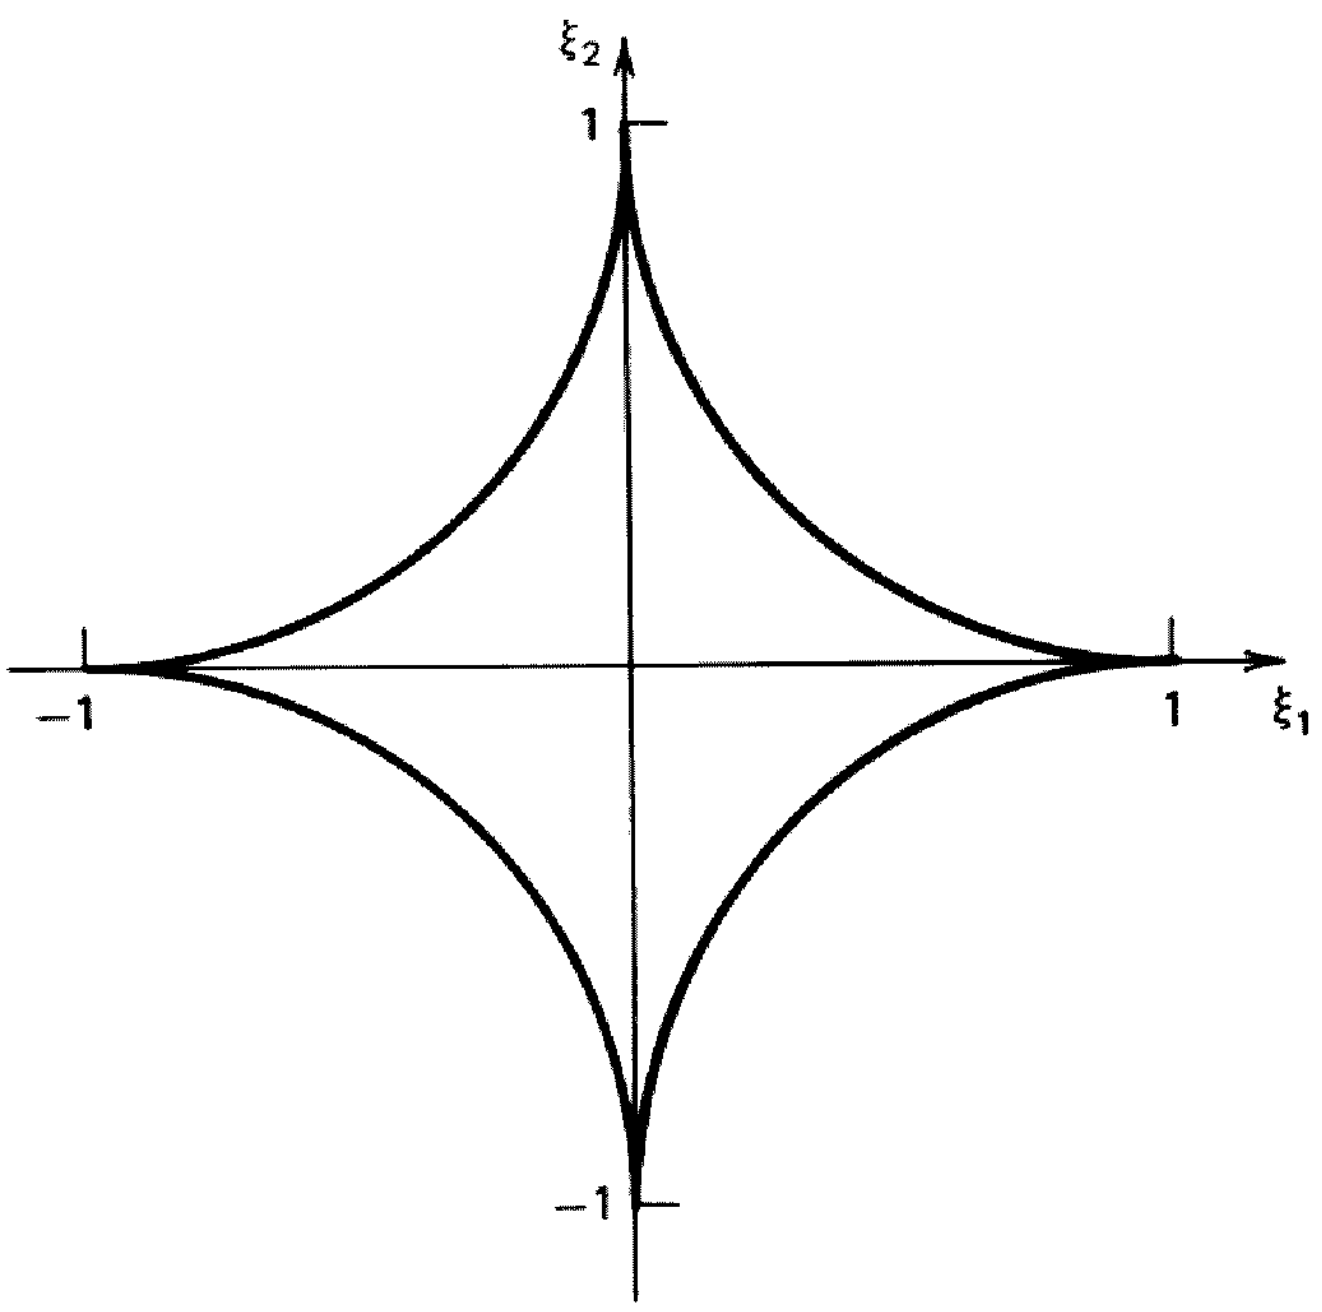
\includegraphics[width=0.5\textwidth]{kreyszig/assets/sec2-2-ex-12.png}
    \caption{Curve $\phi(x)=1$}
    \label{fig:sec2-2-ex12}
\end{figure}
\end{exercise}
\begin{proof}
fill
\end{proof}

\begin{exercise}{13}
fill
\end{exercise}
\begin{proof}
fill
\end{proof}

\begin{exercise}{15 (Bounded set)}
fill
\end{exercise}
\begin{proof}
fill
\end{proof}

\subsection{Further properties of normed spaces}


\begin{exercise}{1}
Show that $c\subseteq l^\infty$ is a vector subspace of $l^\infty$ (cf. 1.5-3) and so is $c_0$, the space of all sequences of scalars converging to zero.
\end{exercise}
\begin{proof}
$c$: Recall that $c$ consists of all convergent sequences. Let $(x^n),(y^n)\in c$ with $x^n\to x$ and $y^n\to y$. Moreover, let $a,b\in\C$. We have $ax^n+by^n\to ax+by$ by the algebraic limit theorem (see, for example, Theorem 2.3.3. of Abbott's understanding analysis), so that $ax^n+by^n\in c$ and hence $c$ is a subspace.

$c_0$: This is a Corollary of the above proof since, if $(x^n),(y^n)\in c_0$, then $x^n\to 0$, $y^n\to 0$ and $ax^n+by^n\to 0$, so that $ax^n+by^n\in c_0$.
\end{proof}

\begin{exercise}{2}
Show that $c_0$ in exercise 1 is a closed subspace of $l^\infty$, so that $c_0$ is complete by 1.5-2 and 1.4-7.
\end{exercise}
\begin{proof}
To prove $c_0$ is closed, we will prove it contains all its limit points. Let $(x^n_m)$ be a convergent sequence where, for each $n$, $x^n\in c_0$, so that $x^n_m\to 0$ (whenever $m\to\infty$), and $x^n_m\to x_m$ (whenever $n\to\infty$). We want to prove $(x_m)\in c_0$.

 We have that for all $\epsilon>0$, there exists an $N\in\N$ so that for all $n>N$, it holds that $d(x^n, x)=\sup_{j=1,\dots}\absoluteValue{x^n_j-x_j}<\epsilon/2$. That is, for all $m$, the difference is less than $\epsilon/2$. Fix this $N$. For the sequence $x^N_m$, for all $\epsilon>0$, there exists $M\in\N$, so that for all $m>M$, it holds that $d(x^N_m, 0)=\absoluteValue{x^N_m}<\epsilon/2$. We then have that $d(x_m,0)\leq d(x_m,x^N_m)+d(x^N_m,0)= \absoluteValue{x_m-x^N_m}+\absoluteValue{x^N_m}=\epsilon$, for $m>M$. Hence, $x_m\to 0$, and $x_m\in c_0$, so that $c_0$ is closed, and by $1.5-2$ and $1.4-7$, complete.
\end{proof}

\begin{exercise}{3}
In $l^\infty$, let $Y$ be the subset of all sequences with only finitely many nonzero terms. Show that $Y$ is a subspace of $l^\infty$ but not a closed subspace.
\end{exercise}
\begin{proof}
Subspace: let $x,y\in Y$, and $a,b$ be scalars. Then both $x$ and $y$ have finitely many nonzero terms, certainly $ax$ and $by$ have finitely many nonzero terms, that is, there exist $N$ and $M$ so that for all $n>N$ and $m>M$ the terms $ax_n$ and $by_m$ are all 0. To see that $ax+by$ has finitely many nonzero terms, notice that for $k>\max[N,M]$ it must be the case that $ax_k+by_k=0$ so that $ax+by\in Y$.

Not closed: in exercise 3 of section 1.5 we defined the sequence (of sequences) given by $x^1=(1,0,0\dots), x^2=(1,1/2,0,\dots), x^3=(1,1/2,1/3,0,\dots),\dots$ and proved that $x^n\to x$ with all the elements of $x$ nonzero. Thus $Y$ is not closed and as a result, not complete.
\end{proof}

\begin{exercise}{4 (Continuity of vector space operations)}
Show that in a normed space $X$, vector addition and multiplication by scalars are continuous operations with respect to the norm; that is, the mappings defined by $(x,y)\to x+y$ and $(\alpha, x)\to \alpha x$ are continuous.
\end{exercise}
\begin{proof}
Addition: Let $x,y,x',y'\in X$. Fix $\epsilon>0$ and let $\delta=\epsilon/2$. We have that if $\norm{(x,y)-(x',y')}_\infty =\max[\norm{x-x'}, \norm{y-y'}] <\delta=\epsilon/2$, then 
\begin{align*}
\norm{f(x,y)-f(x',y)} 
=&\norm{x+y-(x'+y')}\\
\leq& \norm{x-x'}+\norm{y-y'}\\
\leq& 2\max[\norm{x-x'}, \norm{y-y'}] =\epsilon,
\end{align*}
so that addition is continuous.

Scalar multiplication: Let $x,x'\in X$ and $\alpha,\alpha'$ be scalars. Fix $\epsilon>0$ and choose $\delta<\min[1,\epsilon/(1+\absoluteValue{\alpha}+\norm{x})]\leq 1$. We then have that if $\norm{(\alpha, x)-(\alpha',x')}_\infty =\max[\absoluteValue{\alpha-\alpha'}+\norm{x-x'}]<\delta$. Then 
\begin{align*}
    \norm{f(\alpha,x)-f(\alpha',x')} 
    =& \norm{\alpha x-\alpha'x'}\\
    =& \norm{\alpha x-\alpha' x+\alpha' x-\alpha'x'}\\
    =& \norm{\alpha' (x-x')+(\alpha-\alpha')x}\\
    \leq& \norm{\alpha' (x-x')}+\norm{(\alpha-\alpha')x}\\
    =& \absoluteValue{\alpha'}\norm{x-x'}+\absoluteValue{\alpha-\alpha'}\norm{x}\\
    \leq& \absoluteValue{\alpha'}\max[\norm{x-x'}, \absoluteValue{\alpha-\alpha'}]+\norm{x}\max[\norm{x-x'}, \absoluteValue{\alpha-\alpha'}]\\
    =& (\absoluteValue{\alpha'}+\norm{x})\max[\norm{x-x'}, \absoluteValue{\alpha-\alpha'}]\\
    \leq& (\absoluteValue{\alpha'-\alpha}+\absoluteValue{\alpha}+\norm{x})\max[\norm{x-x'}, \absoluteValue{\alpha-\alpha'}]<\epsilon.
\end{align*}
Where the last inequality follows from exercise 3, Section 2.2: $\norm{\alpha'} \leq\norm{\alpha-\alpha'}+\norm{\alpha}$, and the condition that $\delta\leq 1$, so that $\absoluteValue{\alpha-\alpha'}\leq 1$.
\end{proof}

\begin{exercise}{5}
Show that $x^n\to x$ and $y^n\to y$ implies $x^n+y^n\to x+y$. Show that $\alpha^n\to\alpha$ and $x^n\to x$ implies $\alpha^nx^n\to \alpha x$.
\end{exercise}
\begin{proof}
Addition: since $x^n\to x$, then for all $\epsilon>0$, there exists a $N\in\N$ so that for all $n>N$, it holds that $\norm{x^n-x}<\epsilon/2$. Likewise, there exists $N'\in\N$ so that $\norm{y^n-y}<\epsilon/2$ for all $n>N'$. Thus, let $n>\max[N,N']$. We have that $\norm{(x^n+y^n)-(x+y)}\leq \norm{x^n-x}+\norm{y^n-y}<\epsilon$, as required.

Scalar multiplication: since $\alpha^n\to\alpha$, then we have two results. First, $\alpha^n$ is bounded by some constant $A$, so that for all $n$, it holds that $\absoluteValue{\alpha^n}\leq A$. Furthermore, since $\alpha^n\to\alpha$, then for all $\epsilon>0$ there exists an $N\in\N$, so that for all $n>N$, it holds that $\norm{\alpha^n-\alpha}<\epsilon/2\norm{x}$, where $\norm{x}$ is fixed because the limit of $x^n$ is unique. Now,since $x^n\to x$, then for all $\epsilon>0$, there exists an $N'\in\N$ so that for all $n>N$, it holds that $\norm{x^n-x}<\epsilon/2A$.

Thus, let $n>\max[N,N']$. We have that 
\begin{align*}
    \norm{\alpha^nx^n-\alpha x} 
    =& \norm{\alpha^nx^n+\alpha^n x-\alpha^n x -\alpha x}\\
    \leq&\norm{\alpha^n(x^n-x)}+\norm{(\alpha^n-\alpha)x}\\
    =& \absoluteValue{\alpha^n}\norm{x^n-x}+\absoluteValue{\alpha^n-\alpha}\norm{x}\\
    \leq& A\norm{x^n-x}+\absoluteValue{\alpha^n-\alpha}\norm{x}<\epsilon.
\end{align*}
\end{proof}

\begin{exercise}{6}
Show that the closure $\bar{Y}$ of a subspace $Y$ of a normed space $X$ is again a vector subspace.
\end{exercise}
\begin{proof}
Theorem 1.4-6 tells us that $y\in\bar{Y}$ if and only if there is a sequence $(y^n)$ in $Y$ such that $y^n\to y$. Let $x,y\in\bar{Y}$ then there exist sequences $(x^n)$ and $(y^n)$ so that $x^n\to x$ and $y^n\to y$. Furthermore, let $a$ and $b$ be scalars. Because $Y$ is a subspace, we have that $ax^n+by^n\in Y$ for all $n$. Furthermore, from the previous exercise, we know that $ax^n+by^n\to ax+by$, so that $(ax^n+by^n)$ is the required sequence for $ax+by$ to belong to $\bar{Y}$.
\end{proof}

\begin{exercise}{7 (Absolute convergence)}
Show that convergence of $\norm{y^1}+\norm{y^2}+\norm{y^3}+\dots$ may not imply convergence of $y^1+y^2+y^3+\dots$. Hint: Consider $Y$ in exercise 3 and $(y^n)_{n=1,\dots}$ (a sequence indexed by $n$), where $y^n=(y^n_m)_{m=1\dots,}$ (each particular $y^n$ is a sequence indexed by $m$), with $y^n_n=1/n^2$, and $y^n_j=0$ for all $j\neq n$.
\end{exercise}
\begin{proof}
Consider the sequence in the hint, where $Y$ is the subspace of $l^\infty$ where each element of $Y$ has finitely many nonzero elements. The series to evaluate for absolute convergence is given by $\sum 1/n^2$, because $\norm{y^n}=\sup_j\absoluteValue{y^n_j}=1/n^2$. This series of real numbers converges. 

On the other hand, notice that $s^k=y^1+y^2+\dots+y_k$ is the sequence $(1,1/2^2,\dots,1/k^2,0,0,\dots)$. Consider any candidate limit of $s^n$, say $y$. Because $y\in Y$, then there exists an $N\in\N$ so that all elements of $y$ after $N$ are 0. Thus, $\norm{s^k-y}=\sup_j\absoluteValue{s^k_j-y_j}=1/(k+1)^2$, and we cannot get any closer than that value, so that $s^k$ does not converge to $y$. Hence, $s^k$ does not converge in $Y$.
\end{proof}

\begin{exercise}{8}
If in a normed space $X$, absolute convergence of any series always implies convergence of that series, show that $X$ is complete.
\end{exercise}
\begin{proof}
Let $(x^n)$ be a Cauchy sequence in $X$. Then we can construct a subsequence $(x^{n_k})$ so that $\norm{x^{n_{k+1}}-x^{n_k}}<2^{-k}$ for all $k$. Based on this subsequence, consider the sequence given by $x^{n_1}, x^{n_2}-x^{n-1},\dots,x^{n_{k+1}}-x^{n_k},\dots$ and its series in absolute terms:
\[
\norm{x^{n_1}} + \sum_k^\infty \norm{x^{n_{k+1}}-x^{n_k}}
< \norm{x^{n_1}} + \sum_k^\infty 2^k
< \infty.
\]
That is, the series converges absolutely. Then, by assumption, it converges, so that 
\[
x^{n_1} + \sum_k^\infty x^{n_{k+1}}-x^{n_k}
= L <\infty.
\]
Since the sequence telescopes, then for all $\epsilon>0$, there exists an $m\in\N$, so that for all $m>$ it holds that $\norm{x^{n_1} + \sum_k^m x^{n_{k+1}}-x^{n_k} - L} =\norm{x^{n_{m+1}}-L}<\epsilon$. Thus the subsequence converges and by exercise 1.4.2 the original Cauchy sequence converges. Since the Cauchy sequence is arbitrary, $X$ is complete.
\end{proof}

\begin{exercise}{9}
Show that in a Banach space, an absolute convergent series is convergent.
\end{exercise}
\begin{proof}
Let $X$ be Banach and let $(y^n)$ be an absolutely convergent sequence. Let $s^k=\sum^k_j \norm{y^j}$, so that $s^n\to s$. We want to prove that $r^k=\sum^k_j y^j$ converges. Since $(s^n)$ is a sequence of real numbers that converges,  then it is Cauchy, so for all $\epsilon>0$, there exists an $N\in\N$ so that for all $n>m>N$, it holds that
\[
    \norm{s^n-s^m} = \absoluteValue{\sum^n_j \norm{y^j}-\sum^m_j \norm{y^j}} <\epsilon.
\]
But then we have
\begin{align*}
    \absoluteValue{\sum^n_j \norm{y^j}-\sum^m_j \norm{y^j}}
    =& \absoluteValue{\norm{y^n}+\norm{y^{n-1}}+\dots+\norm{y^{m+1}}}\\
    =& \norm{y^n}+\norm{y^{n-1}}+\dots+\norm{y^{m+1}}\\
    \geq& \norm{y^n+y^{n-1}+\dots+y^{m+1}}\\
    =& \norm{r^n-r^m}.
\end{align*}
So that $\norm{r^n-r^m}<\epsilon$ and $(r^n)$ is Cauchy. Since $X$ is complete, then $(r^n)$ converges, so that the series associated with $(y^n)$ is convergent, as required.
\end{proof}

\begin{exercise}{10 (Schauder basis)}
Show that if a normed space has a Schauder basis, it is separable.
\end{exercise}
\begin{proof}
Let $X$ be a normed space with a Schauder basis $e^1,e^2,\dots$. Consider the subset $M$ containing all the finite linear combinations of the basis elements with rational scalars in order, we will call this rational linear combinations. In set notation, $M=\set{\sum_{i=1}^m q^ie^i:q^i\in\Q, m\in\N}$.

We will first prove that $M$ is countable. Consider any $m$ in the above definition. The rational linear combinations are a finite union of countable sets, to see this, notice that the finite sum of can be identified with $\Q\times\dots\times\Q$, $m$ times. Then, since there is a countable number of basis elements, $M$ is the countable union of countable sets, and hence countable.

We will now prove that $M$ is dense in $X$. Let $x\in X$ and fix $\epsilon>0$. Because $e^1,e^2,\dots$ is a Schauder basis, then there exists an $n\in\N$ so that $\norm{x-\sum_{i=1}^n\alpha^ne^n}<\epsilon$, in the definition of Schauder basis, the sequence of $(\alpha^n)$ is a real sequence, however, since the rationals are dense in $\R$, then we can choose rationals so that the same property holds. Notice, however, that this means that our set $M$ is dense in $X$, as such finite sum is contained in $M$. Hence, $X$ is separable, because $M$ is a countable dense subset of $X$.
\end{proof}

\begin{exercise}{11}
Show that $(e^n)$, where $e^n=\delta^n_j$, is a Schauder basis for $l^p$ where $1\leq p<\infty$.
\end{exercise}
\begin{proof}
Let $x\in l^p$ for $1\leq p<\infty$. Then $\sum \absoluteValue{x_j}^p<\infty$, so that $\absoluteValue{x_n}^p\to 0$ (see Abbott Theorem 2.7.3) and because $1\leq p<\infty$, $x_n\to 0$. Let $(\alpha^n)$ be the sequence of scalars corresponding to the entries of $x$. Then $\norm{x-(\alpha^1e^1+\dots+\alpha^ne^n)}=(\sum^\infty_{j=n+1}\absoluteValue{\alpha^j}^p)^{1/p}<\epsilon$, for a suitable choice of $n$. 

Remark: the problem with $p=\infty$ is that $l_\infty$ consists of the bounded sequences and the norm is the supremum of the sequence. Take the sequence of 1s, then there is no $n$ so that the supremum of the difference between the sequence and any potential expansion of the sequence.
\end{proof}

\subsection{Finite dimensional normed spaces and subspaces}


\begin{exercise}{1}
Give examples of subspaces of $l^\infty$ and $l^2$ which are not closed.
\end{exercise}
\begin{proof}
$l^\infty$: We have seen that the subspace $Y$ of $l^\infty$ consisting of all the sequences with finitely many nonzero elements is not closed.

$l^2$: Since the subspace of $l^\infty$ above has finitely many nonzero elements, then it converges under the $p=2$ norm and hence $Y\subseteq l^2$. Thus the example above is an example of a nonclosed subspace of $l^2$.
\end{proof}

\begin{exercise}{3}
Show that in Def. 2.4-4 (Equivalent norms) the axioms of an equivalence relation hold (cf. A1.4 in Appendix 1).
\end{exercise}
\begin{proof}
Let $\norm{\cdot}_1$, $\norm{\cdot}_2$ and $\norm{\cdot}_3$ be norms and $a,a',b$ and $b'$ be constants.

Reflexive: we have $\norm{x}_1 \leq\norm{x}_1 \leq \norm{x}_1$, so that $\norm{x}_1\sim \norm{x}_1$

Symmetric: suppose $\norm{x}_1\sim \norm{x}_2$, that is $a\norm{x}_1 \leq\norm{x}_2 \leq a'\norm{x}_1$, then we have that both $\norm{x}_1\leq (1/a)\norm{x}_2$ and $(1/a')\norm{x}_2 \leq \norm{x}_1$, so that $(1/a')\norm{x}_2 \leq\norm{x}_1 \leq (1/a)\norm{x}_2$, so that $\norm{x}_2 \sim \norm{x}_1$

Transitive: Suppose $\norm{x}_1\sim \norm{x}_2$ and $\norm{x}_2 \sim \norm{x}_3$. That is, $a\norm{x}_1 \leq \norm{x}_2 \leq a'\norm{x}_1$ and $b\norm{x}_2 \leq \norm{x}_3 b'\leq \norm{x}_2$. Thus, $ab\norm{x}_1 \leq b\norm{x}_2 \leq \norm{x}_3$ and $\norm{x}_3 \leq b'\norm{x}_2 \leq a'b'\norm{x}_1$, so that . $ab\norm{x}_1 \leq \norm{x}_3 \leq a'b'\norm{x}_1$. That is, $\norm{x}_1\sim\norm{x}_3$, as required.
\end{proof}

\begin{exercise}{4}
Show that equivalent norms on a vector space $X$ induce the same topology for $X$.
\end{exercise}
\begin{proof}
Let $\norm{\cdot}$ and $\norm{\cdot}_0$ be equivalent in $X$. Then there exist constants $a$ and $b$ so that for all $x\in X$, it holds that $a\norm{x}_0 \leq\norm{x} \leq b\norm{x}_0$.

Let $M$ be an open set in $X$ with respect to $\norm{\cdot}$. Then, for all $x\in M$, there exists an open ball contained in $M$. That is, there exists $r>0$, so that $B(x;ar)\subseteq M$ or, equivalently, if $\norm{x-y}<ar$, then $y\in M$. However, from the definition of equivalence, we have that $a\norm{x-y}_0 \leq\norm{x-y} <r$, thus $M$ is also closed under $\norm{\cdot}_0$. Starting from an open set with respect to $\norm{\cdot}_0$ we can conclude that the set is also open in $\norm{\cdot}$ mutatis mutandis.

Since both norms induce the same open sets, they also induce the same topology, as required.
\end{proof}

\begin{exercise}{5}
If $\norm{\cdot}$ and $\norm{\cdot}_0$ are equivalent norms on $X$, show that the Cauchy sequences in $(X,\norm{\cdot})$ and $(X,\norm{\cdot}_0)$ are the same.
\end{exercise}
\begin{proof}
Let $\norm{\cdot}$ and $\norm{\cdot}_0$ be equivalent in $X$. Then there exist constants $a$ and $b$ so that for all $x\in X$, it holds that $a\norm{x}_0 \leq\norm{x} \leq b\norm{x}_0$.

Let $(x^n)$ be Cauchy in $X$ under $\norm{\cdot}$. Then for all $a,\epsilon>0$, there exists an $N\in\N$ so that for all $n,m>N$, it holds that $a\norm{x^n-x^m}\leq\norm{x^n-x^m}<a\epsilon$, so that $(x^n)$ is also Cauchy in $X$ under $\norm{\cdot}_0$. Starting from a Cauchy sequence under $\norm{\cdot}_0$ we can prove that the sequence is Cauchy under $\norm{\cdot}$ mutatis mutandis.
\end{proof}

\begin{exercise}{8}
Show that the norms $\norm{\cdot}_1$ and $\norm{\cdot}_2$ in exercise 8, Section 2.2, satisfy $1/\sqrt{n}\norm{x}_1\leq\norm{x}_2\leq\norm{x}_1$.
\end{exercise}
\begin{proof}
Recall that $\norm{x}_1=\absoluteValue{x_1}+\dots+\absoluteValue{x_n}$, and $\norm{x}_2=(\absoluteValue{x_1}^2+\dots+\absoluteValue{x_n}^2)^{1/2}$. 

By the Cauchy-Schwarz inequality, we have 
\[
\sum^n_j\absoluteValue{x_j}\leq \sqrt{\sum^n_j\absoluteValue{x_j}^2}\sqrt{\sum^n_j\absoluteValue{1}^2}=\sqrt{\sum^n_j\absoluteValue{x_j}^2}\sqrt{n},
\]
implying the first inequality.

For the second inequality, notice
\[
\norm{x}_1^2 = \absoluteValue{x}^2 = \sum_j^n\sum_i^n\absoluteValue{x_i}\absoluteValue{x_j}\geq \sum_j^n\absoluteValue{x_j}^2 = \norm{x}_2^2.
\]
Taking square root on both sides of the inequality gives us the second inequality.
\end{proof}

\begin{exercise}{9}
If two norms $\norm{\cdot}$ and $\norm{\cdot}_0$ on a vector space $X$ are equivalent, show that (i) $\norm{x^n-x}\to 0$ implies (ii) $\norm{x^n-x}_0\to 0$ (and vice versa, of course).
\end{exercise}
\begin{proof}
Since $\norm{\cdot}$ and $\norm{\cdot}_0$ are equivalent, then there exist constants $a$ and $b$ so that for all $x\in X$, it holds that $a\norm{x}_0 \leq\norm{x} \leq b\norm{x}_0$.

Let $\norm{x^n-x}\to 0$. Then for all $\epsilon>0$, there exists an $N\in\N$ so that for all $n>N$, it holds that $a\norm{x^n-x}_0 \leq\norm{x^n-x} <a\epsilon$. Hence $\norm{x^n-x}_0\to 0$, as required. We can find the other direction by using the same argument mutatis mutandis.
\end{proof}
\subsection{Compactness and finite dimension}

\begin{exercise}{1}
fill
\end{exercise}
\begin{proof}
fill
\end{proof}
\section{Linear operators}


\begin{exercise}{5}
Let $T:X\to Y$ be a linear operator. Show that the image of a subspace $V$ of $X$ is a vector space, and so is the inverse image of a subspace $W$ of $Y$.
\end{exercise}
\begin{proof}
\textbf{Image of the subspace}:

Let $V$ be a subspace of $X$. Let $v,u,w\in V$ and $a,b\in K$. Then we have:

Commutativity: we have $Tv+Tu =T(v+u) = T(u+v) =Tu+Tv$.

Associativity: we have $(Tv+Tu)+Tw =T(v+u)+Tw =T((v+u)+w) =T(v+(u+w)) =Tv+T(u+w) =Tv+(Tu+Tw)$.

Additive identity: we have $Tv+T0 =T(v+0) =Tv$.

Additive inverse: $Tv+T(-v) =T(v-v) =T0 =0$ so that $Tv$ has $T(-v)$ as additive inverse.

Multiplicative identity: we have $1Tv= T(1v) =Tv$ so that 1 is a multiplicative identity.

Distributive properties: we have $(a+b)Tv =T((a+b)v) =T(av+bv) =T(av)+T(bv) =aTv+bTv$. Furthermore, $a(Tv+Tu) =aT(v+u) =T(a(v+u)) =T(av+au) =T(av)+T(au) =aTv+aTu$.

\textbf{Inverse image of a subspace}:

Let $W$ be a subspace of $Y$. Let $v,u,w\in W$, so that $v=Tx, u=Ty, w=Tz$ for $x,y,z\in X$, and $a,b\in K$. Furthermore, notice that because $T$ is a linear operator, it holds that $Tx+Ty =T(x+y)$ and $T(ax) =aTx$. Then we have:

Commutativity: we have $v+u =Tx+Ty =T(x+y) =T(y+x) =Ty+Tx =u+v$.

Associativity: we have $(v+u)+w =(Tx+Ty)+Tz =T(x+y)+Tz =T(x+y+z) =Tx+T(y+z) =Tx+(Ty+Tz) =v+(u+w)$.

Additive identity: since $W$ is a subspace of $Y$, then $0\in W$. Thus, $v+0 =Tx+T0 =T(x+0) =Tx =v$.

Additive inverse:We have $v-v =Tx-Tx =T(x-x) =T0 =0$. So that $v$ has $-v$ as additive inverse.

Multiplicative identity: We have $1v =1Tx =T(1x) =Tx =v$. So that 1 is a multiplicative identity.

Distributive properties: we have $(a+b)v =(a+b)Tx =T[(a+b)x] =T(ax+bx) =T(ax)+T(bx) =aTx +bTx =av+bv$. Likewise, $a(v+u) =a(Tx+Ty) =aT(x+y) =T(a(x+y)) =T(ax+ay) =T(ax)+T(ay) =aTx+aTy =av+au$. 
\end{proof}

\begin{exercise}{6}
If the product (the composite) of two linear operators exist, show that it is linear.
\end{exercise}
\begin{proof}
Let $T:X\to Y$ and $S:Y\to Z$ be linear operators. Then it holds for $TS$:

(i) The domain, $X$, of $TS$ is a vector space and the range $\cR(TS)\subseteq Z$ is a vector space too. Furthermore;

(ii) if $x,x'\in X$, then $T(S(x+x')) =T(Sx+Sx') =TSx+TSx'$, so that $TS$ is additive; and if $a\in K$, then $TS(ax) =T(aSx) =aTSx$ so that $TS$ is homogenous.
\end{proof}

\begin{exercise}{10}
Formulate the conditions in 2.6-10(a) in terms of the null space of $T$.

2.6-10(a): Let $X$ and $Y$ be vector spaces, both real or both complex. Let $T:\cD(T)\to Y$ be a linear operator with domain $\cD(T)\subseteq X$ and range $\cR(T)\subseteq Y$. Then:

(a) The inverse $T^{-1}:\cR(T)\to\cD(T)$ exists if and only if $Tx=0$ implies $x=0$.
\end{exercise}
\begin{proof}
There are two equivalent ways in which we can write this condition: First, the inverse exists, if and only if $\dim\cN(T)=0$. Second, the inverse exists, if and only if $\cN(T)=\set{0}$.
\end{proof}

\begin{exercise}{11}
Let $X$ be the vector space of all $2\times 2$ matrices and define $T:X\to X$ by $Tx=bx$, where $b\in X$ is fixed and $bx$ denotes the usual product of matrices. Show that $T$ is linear. Under what condition does $T^{-1}$ exist?
\end{exercise}
\begin{proof}
Let $x,y\in X$ and $\alpha,\beta\in K$. Then, $T(\alpha x+\beta y) =b(\alpha x+\beta y) =\alpha bx+\beta by =\alpha T(x)+\beta T(y)$, so that $T$ is linear. 

From exercise 10, $T^{-1}$ exists if and only if $\cN(T)=\set{0}$, which is true if and only if $\det b\neq 0$, which is the same as invertible $b$.
\end{proof}

\begin{exercise}{13}
Let $T:\cD(T)\to Y$ be a linear operator whose inverse exists. If $\set{x_1,\dots,x_n}$ is a linearly independent set in $\cD(T)$, show that the set $\set{Tx_1,\dots,Tx_n}$ is linearly independent.
\end{exercise}
\begin{proof}
Consider $0 =a_1Tx_1+\dots+a_nTx_n =T(a_1x_1)+\dots+T(a_nx_n) =T(a_1x_1+\dots+a_nx_n)$. Then we have that $T(a_1x_1+\dots+a_nx_n)=0$, so that $a_1x_1+\dots+a_nx_n=0$. Since $\set{x_1,\dots,x_n}$ is linearly independent, then $a_1=\dots=a_n=0$, so that $\set{Tx_1,\dots,Tx_n}$ is independent too.
\end{proof}

\begin{exercise}{14}
Let $T:X\to Y$ be a linear operator and $\dim X =\dim Y =n <\infty$. Show that $\cR(T)=Y$ if and only if $T^{-1}$ exists.
\end{exercise}
\begin{proof}
($\Rightarrow$) Suppose $\cR(T)=Y$, so that $\dim\cR(T)=\dim Y=n$. Since we assume $X$ and $Y$ are finite dimensional, then the fundamental Theorem of linear algebra which asserts that $\dim X=\dim\cR(T)+\dim\cN(T)$ applies. That is, $n=n+\dim\cN(T)$. Since $\dim\cN(T)=0$, then $T$ is injective, and by 2.6-10.a, then $T^{-1}$ exists.

($\Leftarrow$) Suppose $T^{-1}$ exists. Then by Theorem 2.6-10.c $\dim\cD(T)=\dim X=\dim\cR(T)=\dim Y$, so that $\cR(T)=Y$, because finite dimensional spaces of the same dimension are isomorphic to each other.
\end{proof}

\begin{exercise}{15}
Consider the vector space $X$ of all real-value functions which are defined on $\R$ and have derivatives of all orders everywhere on $\R$. Define $T:X\to X$ by $y(t)=Tx(t)=x'(t)$. Show that $\cR(T)$ is all of $X$ but $T^{-1}$ does not exist. Compare with exercise 14 and comment.
\end{exercise}
\begin{proof}
Since $X$ consists of all the real-valued functions that have derivatives of all orders everywhere on $\R$, then $X$ consists of continuous functions. Thus, we can apply the Fundamental Theorem of Calculus (see Theorem 7.5.1.ii of Abbott) so that if $F\in X$ is differentiable at $x$, then $F(x)=f'(x)$ for some continuous function in $X$. Thus, $\cR(T)=X$. 

To see that $T^{-1}$ does not exist, it suffices to find two functions that have the same preimage under $T$, so that $T$ is not injective. Consider $f(x)=x$ and $g(x)=x+c$ for a constant $c$. Both $f,g\in X$ and $Tf=Tg=1$, so that $T^{-1}1$ is not uniquely defined.

In exercise 14 we assumed the spaces were finite dimensional so we could use the fundamental Theorem of Linear algebra to conclude (starting from the range of $T$) that $T^{-1}$ exists. However, in infnite dimensions this relation between the dimensions of the subspaces does not hold.
\end{proof}
\subsection{Bounded and continuous linear operators}


\begin{exercise}{1}
Let $X,Y,Z$ be normed spaces, and $T_1:Y\to Z$ and $T_2:Y\to Z$ and $T:X\to X$ bounded linear operators. Then:
\begin{enumerate}
    \item $\norm{T_1T_2}\leq\norm{T_1}\norm{T_2}$, and
    \item $\norm{T^n}\leq \norm{T}^n$, for all $n\in\N$.
\end{enumerate}
\end{exercise}
\begin{proof}
Notice that for all $x\in\DDD(T_1,T_2)$ we have
\[
\norm{T_1T_2x}\leq\norm{T_1}\norm{T_2x}\leq\norm{T_1}\norm{T_2}\norm{x},
\]
so that dividing both sides of the inequality by $\norm{x}$ we get that $\norm{T_1T_2}\leq\norm{T_1}\norm{T_2}$, as required.

The second inequality follows from induction, by using $T=T_1=T_2$ in the first step, and $T=T_1$ and $T^{n-1}=T_2$ on the induction step.
\end{proof}

\begin{exercise}{2}
Let $X$ and $Y$ be normed spaces. 
Show that a linear operator $T:X\to Y$ is bounded if and only if $T$ maps bounded sets in $X$ into bounded sets in $Y$.
\end{exercise}
\begin{proof}
($\Rightarrow$) Let $T$ be bounded. Then there exists a constant $c$ so that for all $x\in X$, we have $\norm{Tx}\leq c\norm{x}$. Let $A\subseteq X$ be bounded. Hence, $\sup_{x,y\in A}\norm{x-y}=M<\infty$. Thus, $\norm{T(x-y)}=\norm{Tx-Ty}\leq c\norm{x-y}<\infty$ so that the set $T(A)$ is bounded too.

($\Leftarrow$) Let $T$ map bounded sets to bounded sets, so that if $A\subseteq X$ is a bounded set, then $T(A)\subseteq Y$ is bounded too. Let $A=\set{x\in X:\norm{x}=1}$. To see this is a bounded set, notice that if $x,y\in A$, then $d(x,y)\leq d(x,0)+d(0,y) =\norm{x}+\norm{y}=2$. By exercise 2.2.15, we have that $A$ is bounded if and only if there is a positive number $c$ such that $\norm{x}\leq c$ for all $x\in A$. Thus, since $T(A)$ is bounded, such $c$ exists (notice this is an alternative proof that $A$ itself is bounded, by taking $c=1$). Finally, by definition, we have that $\norm{T} =\sup_{x\in\DDD(T),\norm{x}=1}\norm{Tx} =\sup_{x\in A}\norm{Tx}<\infty$, so that $T$ is bounded, as required.
\end{proof}

\begin{exercise}{5}
Show that the operator $T:l^\infty\to l^\infty$ defined by $x=(x^n)$, $y^n=x^n/n$, $y =(y^n) =Tx$, is linear and bounded.
\end{exercise}
\begin{proof}
We claim that for $\norm{Tx}\leq c\norm{x}$ to hold for all $x\in\l_\infty$ we need to set $c=1$, and thus $T$ is bounded. 
To see this, recall that $l_\infty$ consists of all bounded sequences, so that for all $n$, $\absoluteValue{x^n}\leq M$ for some constant. 
Furthermore, $\norm{x}=\sup_{n\in\N}\absoluteValue{x^n}$. 
We also see that for all $n$, $\absoluteValue{y^n}=\absoluteValue{x^n/n}\leq M$. 
Thus $\sup_{n\in\N}\absoluteValue{x^n/n} =\norm{Tx} \leq\norm{x} =\sup_{n\in\N}\absoluteValue{x^n}$, as required.
\end{proof}

\begin{exercise}{6 (Range)}
Show that the range $\RRR(T)$ of a bounded linear operator $T:X\to Y$ need not be closed in $Y$. 
Hint: Use $T$ in exercise 5.
\end{exercise}
\begin{proof}
Consider the sequence $(x^n)$ given by $x^n=(1,2,\dots,n,0,0,\dots)$. 
Every element of this sequence is in $l^\infty$ (because it is bounded), and the image of every element of the sequence, $T(x^n)=(1,1,\dots,1,0,0,\dots)$ is in $l^\infty$. 
However, the limit of the sequence, the constant sequence of 1s is not in $T(l^\infty)$ because it is the image of the sequence of naturals, $(1,2,\dots,n,n+1,\dots)$ which is not in $l^\infty$ because it is not a bounded sequence.
Hence, $T(l^\infty)$ is not closed.
\end{proof}

\begin{exercise}{7 (Inverse operator)}
Let $T$ be a bounded linear operator from a normed space $X$ onto a normed space $Y$. 
If there is a positive $b$ such that $\norm{Tx}\geq b\norm{x}$ for all $x\in X$, show that then $T^{-1}:Y\to X$ exists and is bounded.
\end{exercise}
\begin{proof}
To see $T$ is injective (and thus has an inverse, given that we assume it is onto), suppose $Tx=Ty$.
Then $0 =\norm{Tx-Ty} \geq b\norm{x-y}\geq 0$, so that $\norm{x-y}=0$ and $x=y$.

To see $T^{-1}$ is bounded, notice that $\norm{x} =\norm{T(T^{-1}x)} \geq b\norm{T^{-1}x}$, so that $(1/b)\norm{x} =c\norm{x} \geq \norm{T^{-1}x}$, as desired.
\end{proof}

\begin{exercise}{8}
Show that the inverse $T^{-1}:\RRR(T)\to X$ of a bounded linear operator $T:X\to Y$ need not be bounded. 
Hint: Use $T$ in exercise 5.
\end{exercise}
\begin{proof}
We argued on exercise 6 that any finite sequence of $n$ sequential 1s is the image of the sequence $(1,2,\dots,n,0,0,\dots)\in l^\infty$.
Now consider the sequence (of sequences), where $x^n$ is the sequence of $n$ 1s.
For each $x^n$, we have $\norm{x^n}_\infty=\sup_j\absoluteValue{x^n_j}=1$.
Furthermore, for all $n$ we have $\norm{T^{-1}x^n} =\sup_j\absoluteValue{nx^n_j} =n$ so
$\norm{T^{-1}}=\sup_{x\in\DDD(T^{-1}),\norm{x}=1}\norm{T^{-1}x}=\infty$, so that $T^{-1}$ is not bounded.
\end{proof}

\begin{exercise}{9}
Let $T:C[0,1]\to C[0,1]$ be defined by $y(t)=\int_0^t x(\tau)d\tau$. 
Find $\RRR(T)$ and $T^{-1}:\RRR(T)\to C[0,1]$. Is $T^{-1}$ linear and bounded?
\end{exercise}
\begin{proof}
We have that $\RRR(T)$ is the set of functions in $[0,1]$ that are differentiable at least once and whose derivative is continuous (that is, in $C^1[0,1]$), and for which $f(0)=0$ (since whenever we integrate with predetermined limits we don't get any constant).
$T^{-1}$ is the differentiation operator, which is linear but not bounded.
To see that $T^{-1}$ is not bounded, notice that $x=t^n$ for an arbitrary $n$, which is in $\RRR(T)$, and use the argument in 2.7-5.
\end{proof}

\begin{exercise}{10}
On $C[0,1]$ define $S$ and $T$ by $y(s)=s\int_0^1x(t)dt$, $y(s)=sx(s)$, respectively. 
Do $S$ and $T$ commute? 
Find $\norm{S}, \norm{T}, \norm{ST}$ and $\norm{TS}$.
\end{exercise}
\begin{proof}
We have 
\begin{align*}
    STx 
    =& S(Tx) = S(sx(s)) = s\int_0^1 tx(t) dt\\
    TSx =& T(Sx) = T(s\int_0^1 x(t) dt) = s^2\int_0^1 x(t)dt.
\end{align*}
So that, in general, $T$ and $S$ do not commute.

Now,
\begin{align*}
    \norm{T} 
    =& \sup_{x\in C[0,1], \norm{x}=1} \norm{Tx}\\
    =& \sup_{x\in C[0,1], \norm{x}=1} \max_{s\in [0,1]}\absoluteValue{sx(s)}\\
    =& \sup_{x\in C[0,1], \norm{x}=1} \max_{s\in [0,1]}\absoluteValue{s}\absoluteValue{x(s)}\\
    \leq& \sup_{x\in C[0,1], \norm{x}=1} \max_{s\in [0,1]}\absoluteValue{s}\max_{s\in [0,1]}\absoluteValue{x(s)}\\
    =& \sup_{x\in C[0,1], \norm{x}=1}\norm{x} =1,
\end{align*}
furthermore, if we take $x(t)=1$ for all $t$, then using equation 3,
\begin{align*}
    1 
    =& \max_{s\in [0,1]}\absoluteValue{sx(s)}
    = \norm{Tx}\\
    \leq& \norm{T}\norm{x}\\
    =& \norm{T}\max_{s\in[0,1]}\absoluteValue{x(s)} =\norm{T}, 
\end{align*}
hence $\norm{T}=1$.

Now for the norm of $S$, we have
\begin{align*}
    \norm{S} 
    =& \sup_{x\in C[0,1], \norm{x}=1}\norm{Sx}\\
    =& \sup_{x\in C[0,1], \norm{x}=1} \max_{s\in[0,1]}\absoluteValue{s\int_0^1x(t)dt}\\
    \leq& \sup_{x\in C[0,1], \norm{x}=1} \max_{s\in[0,1]}\absoluteValue{s} \max_{s\in[0,1]}\absoluteValue{\int_0^1x(t)dt}\\
    =& \sup_{x\in C[0,1], \norm{x}=1} \max_{s\in[0,1]}\absoluteValue{\int_0^1x(t)dt}\\
    \leq& 1.
\end{align*}
The last inequality is true because $\absoluteValue{\int_0^1 x}\leq \int_0^1 \absoluteValue{x}$ and if $x(t)\leq 1$ for all $t$, then $\int_0^1x\leq 1(1-0)$ (Theorem 7.4.2.iii and v in Abbott).
Furthermore, choosing $x(t)=1$ for all $t$ and equation 3,
\begin{align*}
    1 =& \max_{s\in[0,1]}s\int_0^1x(t)dt
    = \max_{s\in[0,1]}\norm{Sx}\\
    \leq& \norm{S}\norm{x}\\
    =& \norm{S}\max_{s\in[0,1]}\int_0^1x(t)dt =\norm{S},
\end{align*}
so that $\norm{S}=1$.

For $\norm{TS}$ and $\norm{ST}$ we can use a similar technique as for $S$ to conclude that $\norm{TS}=\norm{ST}=1$.

\end{proof}

\begin{exercise}{12 (Matrices)}
From 2.7-7 we know that an $r\times n$ matrix $A=(a_{jk})$ defines a linear operator from the vector space $X$ of all ordered $n-$tuples of numbers into the vector space $Y$ of all ordered $r-$tuples of numbers. 
Suppose that any norm $\norm{\cdot}_1$ is given on $X$ and any norm $\norm{\cdot}_2$ is given on $Y$. 
Remember from exercise 2.4.10, that there are various norms on the space $Z$ of all those matrices ($r$ and $n$ fixed). 
A norm $\norm{\cdot}$ on $Z$ is said to be compatible with $\norm{\cdot}_1$ and $\norm{\cdot}_2$ if $\norm{Ax}_2 \leq\norm{A}\norm{x}_1$.

Show that the norm defined by
\[
\norm{A} = \sup_{x\in X, x\neq 0}\frac{\norm{Ax}_2}{\norm{x}_1}
\]
is compatible with $\norm{\cdot}_1$ and $\norm{\cdot}_2$. 
This norm is often called the natural norm defined by $\norm{\cdot}_1$ and $\norm{\cdot}_2$. 
If we choose $\norm{x}_1=\max_j\absoluteValue{x_j}$ and $\norm{y}=\max_j\absoluteValue{y_j}$, show that the natural norm is
\[
\norm{A}=\max_j\sum^n_{k=1}\absoluteValue{a_{jk}}.
\]
\end{exercise}
\begin{proof}
(Compatibility)
We have 
\begin{align*}
    \norm{A}\norm{x'}_1
    =& \sup_{x\in X, x\neq 0}\left\{\frac{\norm{Ax}_2}{\norm{x}_1}\right\}\norm{x'}_1\\
    \geq& \sup_{x\in X, x\neq 0}\left\{\norm{Ax}_2\right\}\frac{\norm{x'}_1}{{\norm{x'}_1}}\\
    =& \sup_{x\in X, x\neq 0}\norm{Ax}_2
    \geq \norm{Ax'}_2,
\end{align*}
as required.

(Natural norm)
We have
\begin{align*}
    \norm{A}
    =& \sup_{x\in X, x\neq 0}\left\{\frac{\max_k \absoluteValue{\sum_l a_{k,l}x_l}}{\max_j \absoluteValue{x_j}}\right\}\\
    \leq& \sup_{x\in X, x\neq 0}\left\{\frac{\max_k \absoluteValue{\sum_l a_{k,l}\max_l \absoluteValue{x_l}}}{\max_j \absoluteValue{x_j}}\right\}\\
    =& \sup_{x\in X, x\neq 0}\left\{\frac{\max_k \absoluteValue{\max_l \absoluteValue{x_l}\sum_l a_{k,l}}}{\max_j \absoluteValue{x_j}}\right\}\\
    =& \sup_{x\in X, x\neq 0}\left\{\frac{\max_l  \absoluteValue{x_l}\max_k\absoluteValue{\sum_l a_{k,l}}}{\max_j \absoluteValue{x_j}}\right\}\\
    =& \sup_{x\in X, x\neq 0}\left\{\max_k\absoluteValue{\sum_l a_{k,l}}\right\}\\
    =& \max_k\absoluteValue{\sum_l a_{k,l}}
\end{align*}
The second inequality would hold be an equality if $x$ is a constant vector.
Choosing $x=(1,\dots,1)$ is enough to get us the desired result.
\end{proof}

\begin{exercise}{13}
Show that in 2.7-7 with $r=n$, a compatible norm is defined by 
\[
\norm{A} = \parens{\sum^n_{j=1}\sum^n_{k=1}a^2_{jk}}^{1/2},
\]
but for $n>1$ this is not the natural norm defined by the Euclidean norm on $R^n$.
\end{exercise}
\begin{proof}
We have 
\begin{align*}
    \norm{Ax}^2
    =& \sum_{j=1}^n \parens{\sum_{k=1}^n a_{jk}x_k}^2\\
    \leq& \sum_{j=1}^n \parens{\sum_{k=1}^n a_{jk}^2}\parens{\sum_{k=1}^n x_k^2}\\
    =& \parens{\sum_{k=1}^n x_k^2}\parens{\sum_{j=1}^n\sum_{k=1}^n a_{jk}^2}\\
    =& \norm{x}^2\norm{A}^2.
\end{align*}
Where the inequality is given by Cauchy-Schwarz applied to every $j$ separately and summing them again. 
Thus, taking square root on both sides of the inequality tells us that $\norm{A}$ is compatible.

To see the second part, consider $A=I$.
Then $\norm{A}=\sqrt{n}$, and the natural norm is 1.
Since they are not the same, then $\norm{A}$ is not the natural norm.
\end{proof}

\begin{exercise}{14}
If in exercise 12 we choose 
\[
\norm{x}_1=\sum^n_{k=1}\absoluteValue{x_k},\quad \norm{y}_2=\sum^r_{j=1}\absoluteValue{y_j},
\]
show that a compatible norm is defined by $\norm{A}=\max_k\sum^r_{j=1}\absoluteValue{a_{jk}}$.
\end{exercise}
\begin{proof}
We have 
\begin{align*}
    \norm{Ax}_2
    =& \sum_j^r \absoluteValue{(Ax)_j}\\
    =& \sum_j^r \absoluteValue{\sum_k^n a_{jk}x_k}\\
    \leq& \sum_j^r \sum_k^n \absoluteValue{a_{jk}x_k}\\
    =& \sum_k^n \absoluteValue{x_k}\sum_j^r \absoluteValue{a_{jk}}\\
    \leq& \sum_k^n \absoluteValue{x_k} \max_k\sum_j^r \absoluteValue{a_{jk}}\\
    =& \sum_k^n \absoluteValue{x_k} \norm{A}\\
    =& \norm{A}\sum_k^n \absoluteValue{x_k} =\norm{A}\norm{x}_1
\end{align*}
Where the first inequality follows from the triangle inequality.
\end{proof}

\begin{exercise}{15}
Show that for $r=n$, the norm in exercise 14 is the natural norm corresponding to $\norm{\cdot}_1$ and $\norm{\cdot}_2$ as defined in that problem.
\end{exercise}
\begin{proof}
Starting from the second equality of exercise 14, we have
\begin{align*}
    \norm{Ax}_2
    =& \sum_j^n \absoluteValue{\sum_k^n a_{jk}x_k}.
\end{align*}
Let $x=(0,\dots,1,\dots,0)$, where $x_k=1$ when $\max_k \sum_j^n \absoluteValue{a_{jk}}$.
Then we have
\begin{align*}
    \sum_j^n \absoluteValue{\sum_k^n a_{jk}x_k}
    &= \sum_j^n \max_k \absoluteValue{a_{jk}}
    = \max_k \sum_j^n\absoluteValue{a_{jk}} = \norm{A}.
\end{align*}
Since $\norm{x}_1=1$, then this is consistent with the natural norm.
If $x_k$ was different from a constant in more than one $k$ then applying the triangle inequality (as the first inequality in exercise 14) would give us that our proposed solution is larger than with the alternative $x$.
\end{proof}
\section{Linear functionals}


\begin{exercise}{2}
Show that the functionals defined on $C[a,b]$ by 
\begin{align*}
    f_1(x) =& \int_a^b x(t)y_0(t)dt\\
    f_2(x) =& \alpha x(a) +\beta x(b),
\end{align*}
for $y_0\in C[a,b]$, and fixed $\alpha,\beta$ are linear and bounded.
\end{exercise}
\begin{proof}
In both cases, let $x,x'\in C[a,b]$ and $c,c'\in \R$.

($f_1$) 
Linear: 
We have 
\begin{align*}
    f_1(cx+c'x') 
    =& \int_a^b(cx(t)+c'x'(t))y_0(t) dt\\
    =& \int_a^b cx(t)y_0(t)dt + \int_a^b c'x'(t)y(t)_0dt\\
    =& c\int_a^b x(t)y_0(t)dt + c'\int_a^b x'(t)y(t)_0dt\\
    =& cf_1(x)+c'f_1(x').
\end{align*}

Bounded: 
We have
\begin{align*}
    \norm{f_1(x)}
    =& \absoluteValue{\int_a^b x(t)y_0(t)dt}\\
    \leq& \int_a^b \absoluteValue{x(t)y_0(t)}dt\\
    \leq& \int_a^b \absoluteValue{x(t)}\absoluteValue{y_0(t)}dt\\
    \leq& \int_a^b \max_{s\in[a,b]}\absoluteValue{x(s)}\absoluteValue{y_0(t)}dt\\
    &= \max_{s\in[a,b]}\set{\absoluteValue{x(s)}} \int_a^b\absoluteValue{y_0(t)}dt =\norm{x}c.
\end{align*}

($f_2$)
Linear:
We have
\begin{align*}
    f_2(cx +c'x')
    =& \alpha [cx(a)+c'x'(a)] +\beta [cx(b)+c'x'(b)]\\
    =& c\alpha x(a)+ c'\alpha x'(a) 
    +c\beta x(b) + c'\beta x'(b)\\
    =& c[\alpha x(a) +\beta x(b)]
    + c'[\alpha x'(a) +\beta x'(b)] = cf_2(x)+c'f_2(x'),
\end{align*}
so that $f_2$ is linear.

Bounded:
We have
\begin{align*}
    \norm{f_2(x)}
    =& \absoluteValue{\alpha x(a) +\beta x(b)}\\
    \leq& \absoluteValue{\alpha x(a)} 
    +\absoluteValue{\beta x(b)}\\
    =& \absoluteValue{\alpha}\absoluteValue{x(a)} 
    +\absoluteValue{\beta}\absoluteValue{x(b)}\\
    \leq& \absoluteValue{\alpha}\absoluteValue{\max_{t\in [a,b]}x(t)} 
    +\absoluteValue{\beta}\absoluteValue{\max_{t\in [a,b]}x(t)}\\
    =& (\absoluteValue{\alpha}+\absoluteValue{\beta})\absoluteValue{\max_{t\in [a,b]}x(t)}\\
    \leq& (\absoluteValue{\alpha}+\absoluteValue{\beta})\max_{t\in [a,b]}\absoluteValue{x(t)} = c\norm{x}.
\end{align*}
\end{proof}

\begin{exercise}{4}
Show that $f_1(x)=\max_{t\in J} x(t)$ and $f_2(x)=\min_{t\in J} x(t)$ for $J=[a,b]$ define functionals on $C[a,b]$. 
Are they linear? Bounded?
\end{exercise}
\begin{proof}
($\max$)
The $\max$ functional is not linear.
Consider $f,g\in C[a,b]$ given by $x(t)=1$ if $t\in[a,(a+b)/2]$ and $x(t)=0$ otherwise, and $y(t)=0$ if $t\in[a,(a+b)/2]$ and $y(t)=1$ otherwise.
Then $f_1(x+y)=1$, but $f_1(x)+f_1(y)=2$.

The $\max$ functional is bounded.
To see this, notice that 
\begin{align*}
\norm{f_1(x)} =\absoluteValue{\max_{t\in J}x(t)} \leq\max_{t\in J}\absoluteValue{x(t)} =\norm{x},    
\end{align*}
as required.

($\min$)
We can prove that $\min$ is not linear using the same functions as with $\max$.
In that case, we would obtain $f_2(x+y) =1$ and $f_2(x)+f_2(y)=0$.

$\min$ is bounded.
To see this, we have 
\begin{align*}
    \norm{f_2(x)} 
    =\absoluteValue{\min_{t\in J}x(t)} 
    \leq \max_{t\in j}\absoluteValue{x(t)}
    =\norm{x}.
\end{align*}
\end{proof}

\begin{exercise}{5}
Show that on any sequence space $X$ we can define a linear functional $f$ by setting $f(x)=x_n$ ($n$ fixed, where $x=(x_n)$. 
Is $f$ bounded if $X=l^\infty$?
\end{exercise}
\begin{proof}
$f$ is bounded, since $l^\infty$ consists of all bounded sequences, and the norm in $l^\infty$ is defined as the supremum of the sequence.
Thus, for any $n$, $\norm{fx} =\absoluteValue{x_n}\leq \sup_n\absoluteValue{x_n} =\norm{x}$.
\end{proof}

\begin{exercise}{6 (Space $C^1[a,b]$)}
The space $C^1[a,b]$ or $C'[a,b]$ is the normed space of all continuously differentiable functions on $J=[a,b]$ with norm defined by $\norm{x}=\max_{t\in J}\absoluteValue{x(t)}+\max_{t\in J}\absoluteValue{x'(t)}$. Show that the axioms of a norm are satisfied. 
Show that $f(x)=x'(c)$, $c=(a+b)/2$, defines a bounded linear functional on $C^1[a,b]$. 
Show that $f$ is not bounded, considered as a functional on the subspace of $C[a,b]$ which consists of all continuously differentiable functions.
\end{exercise}
\begin{proof}
($\norm{x}$ is a norm)

i) Since we are taking $\max$ of absolute values, the norm is necessarily greater than or equal to 0.

ii) Equality of the previous point only holds whenever the function is the 0 function, since otherwise the $\max$ would be greater than 0.

iii) Let $a\in\R$ and $x\in C^1[a,b]$. Then we have that 
\begin{align*}
\norm{a x} 
=& \max_{t\in J}\absoluteValue{a x(t)} 
+ \max_{t\in J}\absoluteValue{a x'(t)}\\
=& \absoluteValue{a}\max_{t\in J}\absoluteValue{x(t)} 
+ \absoluteValue{a}\max_{t\in J}\absoluteValue{x'(t)}\\
=& \absoluteValue{a}[\max_{t\in J}\absoluteValue{x(t)} 
 + \max_{t\in J}\absoluteValue{x'(t)}] = \absoluteValue{a}\norm{x}.
\end{align*}

vi) Furthermore, if $y\in C^1[a,b]$, we have
\begin{align*}
    \norm{x+y}
=& \max_{t\in J}\absoluteValue{x(t) + y(t)} 
+ \max_{t\in J}\absoluteValue{(x(t) +y(t))'}\\
=& \max_{t\in J}\absoluteValue{x(t) + y(t)} 
+ \max_{t\in J}\absoluteValue{x'(t) + y'(t)}\\
\leq& \max_{t\in J}\set{\absoluteValue{x(t)} + \absoluteValue{y(t)}}
+ \max_{t\in J}\set{\absoluteValue{x'(t)} + \absoluteValue{y'(t)}}\\
\leq& \max_{t\in J}\absoluteValue{x(t)} 
+ \max_{t\in J}\absoluteValue{y(t)}
+ \max_{t\in J}\absoluteValue{x'(t)} 
+ \max_{t\in J}\absoluteValue{y'(t)}\\
& [\max_{t\in J}\absoluteValue{x(t)} 
+ \max_{t\in J}\absoluteValue{x'(t)}]
+ [\max_{t\in J}\absoluteValue{y(t)}
+ \max_{t\in J}\absoluteValue{y'(t)}] 
=\norm{x}+\norm{y}.
\end{align*}

($f$ linear and bounded functional in $C^1[a,b]$)

Linear.
Let $x,y\in C^1[a,b]$ and $a,b\in\R$.
We have 
\begin{align*}
f(ax+by) 
=& (ax+by)'(c)\\
=& (ax)'(c)+(by)'(c)\\
=& ax'(c)+by'(c) =af(x)+bf(y).
\end{align*}


Bounded.
We have 
\begin{align*}
\norm{fx} 
=& \absoluteValue{x'(c)}\\
\leq& \max_{t\in J}\absoluteValue{x'(t)}\\
\leq& \max_{t\in J}\absoluteValue{x(t)} + \max_{t\in J}\absoluteValue{x'(t)} =\norm{x}.
\end{align*}

($f$ not bounded when defined on the subspace of continuously differentiable functions of $C[a,b]$)
To see $f$ is not bounded when considered as a functional on the subspace of $C[a,b]$, consider the sequence of functions $x_n(t)=\arctan(nt)/n$ in $C[0,1]$.
We have
\begin{align*}
    \norm{x}
    = \max_{t\in[0,1]}\absoluteValue{\arctan(nt)/n} \to 0,
\end{align*}
as $n\to\infty$, given that $\arctan{x}\leq\pi/2$.
On the other hand,
\begin{align*}
    \norm{f(x)}
    = \absoluteValue{1/(n^2x^2+1)} \to 1,
\end{align*}
as $n\to\infty$.
Thus we cannot find a $c\in\R$ with $\norm{f(x_n)}\leq c\norm{x_n}$, given that for any $c$, we can find an $N$ so that the equality does not hold for any $n>N$.
Thus, the functional $f$ is not bounded, when thinking of $x$ as a subspace of $C[0,1]$.
\end{proof}

\begin{exercise}{7}
If $f$ a bounded linear functional on a complex normed space, is $\bar{f}$ Bounded? Linear?
(The bar denotes complex conjugate).
\end{exercise}
\begin{proof}
(Linear)
$\bar{f}$ is not linear. 
To see this, consider $x,y\in X$ and $a,b\in\C$.
Then, 
\begin{align*}
    \bar{f}(ax) 
    =\overline{f(ax)} 
    =\bar{a}\overline{f(x)},
\end{align*}
which does not equal $a\overline{f(x)}$ in the generic case, so that $\bar{f}$ is not homogenous and thus not linear.

(Bounded)
$\bar{f}$ is bounded.
We have
\begin{align*}
\norm{\bar{f}(x)}
= \absoluteValue{\bar{f}(x)}
= \absoluteValue{f(x)}
\leq c\norm{x},
\end{align*}
where the inequality follows because $f$ is bounded.
\end{proof}

\begin{exercise}{9}
Let $f\neq 0$ be any linear functional on a vector space $X$ and $x_0$ any fixed element of $X\setminus \cN(f)$, where $\cN(f)$ is the null space of $f$.
Show that any $x\in X$ has a unique representation $x=\alpha x_0+y$, where $y\in\cN(f)$.
\end{exercise}
\begin{proof}
Theorem 1.45 in Axler's Linear Algebra says that the sum of two subspaces of $X$ is a direct sum if and only if the intersection of the subspaces is zero.
That condition is precisely satisfied for the subspaces $\vecspan(x_0)$ and $\cN(f)$.
Since $x_0\in X\setminus\cN(f)$, then $f(\alpha x_0)\neq 0$ for $\alpha\neq 0$ and $f(\alpha x_0)=0$ if $\alpha=0$, thus $\vecspan(x_0)\cap \cN(f)=\set{0}$.

Now to see that $x\in X$ can be represented as such, choose $\alpha = f(x)/f(x_0)$ and $y=x-\alpha x_0$.
Since $x_0\in X\setminus\cN(f)$, then $\alpha$ is defined and $f(y) =f(x-\alpha x_0) =f(x)-\alpha f(x_0) =f(x)-f(x)=0$, so that $y\in\cN(f)$.
Last, we have $\alpha x_0+y =\alpha x_0 +x-\alpha x_0=x$, as required.
\end{proof}

\begin{exercise}{10}
Show that in exercise 9, two elements $x_1,x_2\in X$ belong to the same element of the quotient space $\quot{X}{\cN(f)}$ if and only if $f(x_1)=f(x_2)$;
show that $\text{codim }\cN(f)=1$.
(Cf. 2.1.14).
\end{exercise}
\begin{proof}
Recall that $x_1$ and $x_2$ are equivalent if and only if $x_1-x_2\in\cN(f)$.
Suppose $x_1$ and $x_2$ belong to the same element of the quotient space.
Then $x_1+y_1=x_2+y_2$ for $y_1,y_2\in\cN(f)$, but this implies $f(x_1+y_1) =f(x_1)+f(y_1) =f(x_1) =f(x_2+y_2) =f(x_2)$, as required.

Now suppose $f(x_1)=f(x_2)$.
Then $f(x_1)-f(x_2) =f(x_1-x_2) =0$, so that $x_1-x_2\in\cN(f)$, so that they are elements of the quotient space.

Too see $\text{codim }\cN(f)=1$ we use the result we just proved.
That is, we just proved that the points in $X$ are collapsed to elements in the codomain in $f$, the reals.
Since the reals is a one-dimensional vector space, then the quotient space (and the codimension of $f$) are one dimensional too.
\end{proof}

\begin{exercise}{11}
Show that two linear functionals $f_1\neq 0$ and $f_2\neq 0$ which are defined on the same vector space and have the same null space are proportional.
\end{exercise}
\begin{proof}
This is a corollary to exercise 9.
The definition of direct sum (see 1.40 in Axler) tells us that each element of the sum can be written in only one way as the sum of elements of each of the subspaces.
Since $\cN(f_1)=\cN(f_2):=\cN(f)$, for a fixed $x_0$, every $x\in X$ can be written as $x=\alpha x_0+y$, where $y\in\cN(f)$, with a unique $\alpha$.
The choice of $\alpha$ we found in exercise 9 is $\alpha=f_1(x)/f_1(x_0)=f_2(x)/f_2(x_0)$.
Since $x_0$ is fixed before hand, this implies $cf_1(x)=f_2(x)$, where $c=f_2(x_0)/f_1(x_0)$, giving us the desired result.
\end{proof}

\begin{exercise}{12 (Hyperplane)}
If $Y$ is a subspace of a vector space $X$ and $\text{codim }Y=1$ (cf. 2.1.14), then every element of $\quot{X}{Y}$ is called a hyperplane parallel to $Y$.
Show that for any linear functional $f\neq 0$ on $X$, the set $H_1=\set{x\in X: f(x)=1}$ is a hyperplane parallel to the null space $\cN(f)$ of $f$.
\end{exercise}
\begin{proof}
This is a Corollary to exercise 10.
Since all elements of $x_1$ and $x_2$ of $H_1$ map to the same value under $f$, then they belong to the same element of the quotient space.
$H_1$ constitutes the whole element of $\quot{X}{\cN(f)}$ because any other $x$ whose value under $f$ would be different would belong to another element of the quotient space.
\end{proof}

\begin{exercise}{13}
If $Y$ is a subspace of a vector space $X$ and $f$ is a linear functional on $X$ such that $f(Y)$ is no the whole scalar field of $X$, show that $f(y)=0$ for all $y\in Y$.
\end{exercise}
\begin{proof}
Suppose there exists $y\in Y$ so that $f(y)\neq 0$.
Then since $f$ is linear and homogenous, and $Y$ is a vector space itself, then for all $k$ in the scalar field we can choose $a=k/f(y)$, so that $f(ay)=af(y)=k$.
Now if $Y\subseteq\cN(f)$, then $f(y)=0$ for all $y\in Y$, and $f$ would still be a valid functional on $X$.
\end{proof}

\begin{exercise}{14}
Show that the norm $\norm{f}$ of a bounded linear functional $f\neq 0$ on a normed space $X$ can be interpreted geometrically as the reciprocal of the distance $\bar{d}=\inf\set{\norm{x}: f(x)=1}$ of the hyperplane $H_1=\set{x\in X: f(x)=1}$ from the origin.
\end{exercise}
\begin{proof}
Notice that, by definition, $\norm{f}$ is the smallest $c$ (the infimum) such that $\norm{f(x)x}/\norm{f}\leq c$.
Now let $x\in H_1$, thus, $f(x)=1$ and so $1/\norm{x}\leq c$.
Since the quantity on the left is maximised whenever $\norm{x}$ is the minimised, then $\norm{f}$ is the inverse (or reciprocal) of $\bar{d}=\inf\set{\norm{x}:f(x)=1}$, as required.
\end{proof}
\subsection{Linear operators and functional on finite dimensional spaces}

\begin{exercise}{1}
fill
\end{exercise}
\begin{proof}
fill
\end{proof}
\section{Normed spaces of operators. Dual space}


\begin{exercise}{1}
What is the zero element of the vector space $B(X,Y)$?
The inverse of a $T\in B(X,Y)$ in the sense of Definition 2.1-1?
\end{exercise}
\begin{proof}
(Zero element of $B(X,Y)$) 
The zero element of $B(X,Y)$ is the linear map that $T$ such that for every $x\in X$, $Tx=0$.

(Inverse of $T$)
The inverse of $T$ is simply $-T$.
By linearity, we have $T + (-T)x= Tx + (-Tx) = Tx - Tx = 0$.
\end{proof}

\begin{exercise}{2}
The operators and functionals considered in the text are defined on the entire space $X$.
Show that without that assumption, in the case of functionals we still have the following theorem:
If $f$ and $g$ are bounded linear functionals with domains in a normed space $X$ then for any nonzero scalars $\alpha$ and $\beta$ the linear combination $h=\alpha f+\beta g$ if a bounded linear functional with domain $\cD(f)\cap\cD(g)$.
\end{exercise}
\begin{proof}
Let $f$ be a bounded linear functional with domain $\cD(f)$ and $g$ a bounded linear functional with domain $\cD(g)$.
Furthermore, let $\alpha, \beta, a, b$ be nonzero scalars.
For $x,y \in\cD(f)\cap\cD(g)$, we have:
\begin{align*}
    h(ax+by) 
    =& \alpha f(ax+by) + \beta g(ax+by)\\
    =& \alpha af(x)+ \alpha bf(y) + \beta ag(x) + \beta bg(y)\\
    =& a[\alpha f(x) + \beta g(x)] + b[\alpha f(y) + \beta g(y)]\\
    =& ah(x) + bh(y),
\end{align*}
so that $h$ is a linear functional

Now, to see $h$ is bounded, we have 
\begin{align*}
    \absoluteValue{h(x)} 
    =& \absoluteValue{\alpha f(x) + \beta g(x)}\\
    \leq& \absoluteValue{\alpha f(x)} + \absoluteValue{\beta g(x)}\\
    =& \absoluteValue{\alpha}\absoluteValue{f(x)} + \absoluteValue{\beta}\absoluteValue{g(x)}\\
    \leq& \absoluteValue{\alpha}c\norm{x} + \absoluteValue{\beta}c'\norm{x}\\
    =& [\absoluteValue{\alpha}c + \absoluteValue{\beta}c']\norm{x},
\end{align*}
as required.
Here $c$ is the constant for which $\absoluteValue{f(x)} \leq c\norm{x}$ for all $x$, and likewise for $c'$ and $g$.
\end{proof}

\begin{exercise}{3}
Extend the Theorem in exercise 2 to bounded linear operators $T_1$ and $T_2$.
\end{exercise}
\begin{proof}
The proof above does not depend on $f$ or $g$ being functionals but on their linear and bounded nature.
\end{proof}

\begin{exercise}{4}
Let $X$ and $Y$ be normed spaces and $T_n:X\to Y\ (n=1,2\dots)$ bounded linear operators.
Show that convergence $T_n\to T$ implies that for every $\epsilon>0$ there is an $N$ such that for all $n>N$ and all $x$ in any given closed ball we have $\norm{T_nx-Tx} <\epsilon$.
\end{exercise}
\begin{proof}
Consider a closed ball $B$ and let $k =\sup_{x\in B}\norm{x}<\infty$, because a closed ball is bounded.
Let $\epsilon >0$, then there exists $N \in\N$, such that for all $n>N$, it holds that $\norm{T_n-T} <\epsilon/k$.
Because $T_n$ and $T$ are bounded, $T_n-T$ is bounded and then the following holds
\begin{align*}
    \norm{T_nx-Tx} 
    = \norm{(T_n-T)x}
    \leq \norm{T_n-T}\norm{x}
    < \epsilon\norm{x}/k <\epsilon,
\end{align*}
Giving us the desired result.
\end{proof}

\begin{exercise}{6}
If $X$ is the space of ordered $n$-tuples of real numbers and $\norm{x}=\max_i \absoluteValue{x_i}$, what is the corresponding norm on the dual space $X'$?
\end{exercise}
\begin{proof}
Following the examples in the section, we are going to consider the functional given by $f(x) =\sum_i^n x_i\gamma_i$, where $\gamma_i = f(e_i)$ for a basis $e_1,\dots,e_n$ of $X$.
We then have
\begin{align*}
    \absoluteValue{f(x)}
    =& \absoluteValue{\sum_i^n x_i\gamma_i}.
\end{align*}
Choose $x_i = 1$ if $\gamma_i>0$ and $x_i = -1$ if $\gamma_i \leq 0$, so that we will obtain:
\begin{align*}
    \absoluteValue{\sum_i^n \gamma_i}
    =& \sum_i^n\absoluteValue{\gamma_i} = \norm{\gamma}_1
\end{align*}
and because $x$ is a sequence of $-1$ or $1$, then $\norm{x}_\infty=1$ so that $\norm{f} = \norm{\gamma}_1$, giving us the desired result.
\end{proof}

\begin{exercise}{8}
Show that the dual space of the space $c_0$ is $l^1$. 
(See exercise 2.3.1).
\end{exercise}
\begin{proof}
We will divide this proof in 2 steps:

(For any $f\in c_0'$ we have $f\in l_1$)
Suppose $f$ is a bounded functional in $c_0'$ and let $x\in c_0$.
Then
\begin{align*}
    f(x) = \sum x_iy_i,
\end{align*}
where $y_i=f(e_i)$ and $(e_n)$ is a Schauder basis of $c_0$.
Since $f$ is bounded, we have that for any choice $x\in c_0$ with $\norm{x}_\infty$
\begin{align*}
    \absoluteValue{f(x)}
    = \absoluteValue{\sum x_iy_i}
    \leq \norm{f},
\end{align*}
where $y_i=f(e_i)$ and $(e_n)$ is a Schauder basis of $c_0$.
Now choose $x_i = \sgn(y_i)$ if $i\leq N$ for $N\in \N$, and 0 otherwise.
We then obtain
\begin{align*}
    \absoluteValue{\sum^N_i x_iy_i}
    = \sum^N_i y_i
    = \sum^N_i \absoluteValue{y_i}
    \leq \norm{f},
\end{align*}
and taking $N\to\infty$, we get that $y_i\in l_1$.
This choice of $x$ gives us the supremum of $\norm{f(x)}$ for $x$ with norm 1, so that the norm in $c_0'$ is indeed the 1-norm.

(For some $y\in l_1$ we can find a bounded functional in $c_0'$)
Let $y\in l_1$ and define a functional on $c_0$ in the natural way:
\begin{align*}
    f(x) = \sum^\infty_i x_iy_i.
\end{align*}
We then have
\begin{align*}
    \absoluteValue{f(x)}
    =& \absoluteValue{\sum^\infty_i x_iy_i}\\
    \leq& \absoluteValue{\sum^\infty_i \max_j \absoluteValue{x_j}y_i}\\
    \leq& \sum^\infty_i \absoluteValue{\max_j \absoluteValue{x_j}y_i}\\
    =& \max_j \absoluteValue{x_j}\sum^\infty_i \absoluteValue{y_i}\\
    =& \norm{x}_\infty\norm{y}_1,
\end{align*}
as required.
\end{proof}

\begin{exercise}{9}
Show that a linear functional $f$ on a vector space $X$ is uniquely determined by its values on a Hamel basis for $X$.
(See section 2.1).
\end{exercise}
\begin{proof}
Let $f$ be a linear functional on $X$ and let $e_1,\dots,e_n$ be a basis of $X$.
Suppose, for the sake of contradiction, that there exists another linear functional $f'$ so that for all $e_i$, $f(e_i)=f'(e_i)$.
Now let $x\in X$ so that we can write $x = a_1e_1+\dots+a_ne_n$ where all $a_i$ are unique.
We have 
\begin{align*}
f(x) 
=& f(a_1e_1+\dots+a_ne_n)\\
=& a_1f(e_1)+\dots+a_nf(e_n)\\
=& a_1f'(e_1)+\dots+a_nf'(e_n)\\
=& f'(a_1e_1+\dots+a_ne_n)
= f'(x),
\end{align*}
so that $f$ and $f'$ are not distinct.
\end{proof}

\begin{exercise}{10}
Let $X$ and $Y\neq\set{0}$ be normed spaces, where $\dim X=\infty $.
Show that there is at least one unbounded linear operator $T:X\to Y$.
(Use a Hamel basis).
\end{exercise}
\begin{proof}
Consider the space $W\subseteq l_1$, where $W$ consists of all sequences with finitely many nonzero values.
We start our definition of $f$ by mapping all $w\in W$ to 0.
Take the set $\set{(1,0,0,\dots), (0,1,0,\dots), (0,0,1,0,\dots),\dots}\subseteq W$ and extend it to a Hamel basis of $l_1$.
The elements that compose the extension of the set above are mapped by $f$ to 1.
By exercise 9, this defines a unique functional on $l_1$.
Consider the sequence of sequences in $l_1$ where the $i$-th sequence $(x_n^i)\in l_1$ is given by $x_k = 1/k^2$ if $k\leq i$ and 0 otherwise.
We have that $(x^i_n)\to (x_n)$, where $x_n=1/n^2$.
For each $i$, $f(x^i) = f(\sum^i_{k=1} (1/k^2)e_k) = \sum^i_{k=1} (1/k^2)f(e_k) = 0$.
However, from our definition of $f$, we know that $f(x)\neq 0$, because $x$ is not a finite linear combination of the set we extended to be a Hamel basis of $l_1$.
Thus, $f$ is not continuous (given that $0 = \lim_n f(x^n) \neq f(\lim_n x^n) = f(x)$), and by Theorem 2.7-9, $f$ is not bounded.
\end{proof}

\begin{exercise}{11}
If $X$ is a normed space and $\dim X=\infty$, show that the dual space $X'$ is not identical with the algebraic dual space $X^\ast$.
\end{exercise}
\begin{proof}
The previous exercise is as an example of this, as the dual space is the space of bounded linear functionals, and we saw that there is an unbounded functional in $l_1$.
\end{proof}

\begin{exercise}{12 (Completeness)}
The examples in the text can be used to prove completeness of certain spaces.
How?
For what spaces?
\end{exercise}
\begin{proof}
In the examples we proved that $l_p'$ and $l_q$ are isomorphic and that $l_1'$ and $l_\infty$ are isomorphic so that if we can prove that $l_p'$ and $l_1'$ are complete, then $l_q$ and $l_\infty$ are complete too.
However, Theorem 2.10-4 tells us that the dual space of a normed space is Banach, giving us the completeness that we wanted.
\end{proof}


\section{Inner product spaces. Hilbert spaces}
\subsection{Inner product space. Hilbert space}

\begin{exercise}{1}
fill
\end{exercise}
\begin{proof}
fill
\end{proof}
\subsection{Further properties of inner product spaces}

\begin{exercise}{1}
fill
\end{exercise}
\begin{proof}
fill
\end{proof}
\section{Orthogonal complements and direct sums}

3 Simple example to reinforce the ideas
9
10 Two very important theorems related to the orthogonal complement and double complement. Used all the time!

\begin{exercise}{1}
Let $H$ be a Hilbert space, $M \subseteq H$ a convex subset, and $(x_n)$ a sequence in $M$ such that $\norm{x_n} \to d$, where $d = \inf_{x \in M} \norm{x}$.
Show that $(x_n)$ converges in $H$.
Give an illustrative example in $\R^2$ or $\R^3$.
\end{exercise}
\begin{proof}
We will follow a strategy similar to Theorem 3.3-1.
To do that, we will prove $(x_n)$ is Cauchy, and then it will follow by the completeness of $H$, that $(x_n)$ converges in $H$.
Let $\norm{x_n} = d_n$.
We have that $\norm{x_n + x_m} = 2\norm{1/2(x_n + x_m)} \geq 2d$, because $x_n/2 + x_m/2$ is in $M$ due to its convexity.
Now by the parallelogram equality, we have that
\begin{align*}
    \norm{x_n - x_m} 
    =& -\norm{x_n + x_m}^2 + 2(\norm{x_n} + \norm{x_m})\\
    \leq& -(2d)^2 + 2(d_n + d_m) \to 0,
\end{align*}
where the convergence to 0 follows from the fact that $d_n,d_m \to d$.
Thus $(x_n)$ is Cauchy and by the completeness of $H$ it must converge to a point in $H$.
\end{proof}

\begin{exercise}{2}
Show that the subset $M=\set{y=(y_i): \sum y_i=1)}$ of complex space $\C^n$ (see 3.1-4) is complete and convex.
Find the vector of minimum norm in $M$.
\end{exercise}
\begin{proof}
(Complete)
Let $(x^n)$ be a sequence (of sequences) in $M$, so that for each sequence, $\sum_i x^n_i=1$.
Assume $x^n\to x$, so that for every $\epsilon>0$, we can find an $n\in\N$ such that $\norm{x^n-x}_1<\epsilon$.
We have
\begin{align*}
    \absoluteValue{1-\sum_i x_i}
    =& \absoluteValue{\sum_i x^n_i - \sum_i x_i}\\
    =& \absoluteValue{\sum_i x^n_i - x_i}\\
    \leq& \sum_i\absoluteValue{x^n_i - x_i}
    <\epsilon.
\end{align*}
That is, $x\in M$
Theorem 1.4-6 states that a closed subset of a complete space is complete.
Since $\C^n$ is complete, and $M$ is closed, then $M$ is complete.

(Convex)
For $x,y\in M$ and $a\in[0,1]$, we have
\begin{align*}
    \sum_i (ax_i+(1-a)y_i)
    =& \sum_i ax_i + \sum_i (1-a)y_i\\
    =& a\sum_i x_i + (1-a)\sum_i y_i\\
    =& a + (1-a) = 1,
\end{align*}
so that $ax+(1-a)y\in M$.

(Vector of minimum norm)
The norm of a vector $x$ in $\C^n$ is $\sum_i x_i\bar{x}_i$.
The vector that minimises such norm is $x_i=1/n$ for all $i$.
\end{proof}

\begin{exercise}{3}
\begin{enumerate}
    \item Show that the vector space $X$ of all real-valued continuous functions on $[-1,1]$ is the direct sum of of the set of all even continuous functions and the set of all odd functions on $[-1,1]$.
    \item Give examples of representations of $\R^3$ as a direct sum (i) of a subspace and its orthogonal complement, (ii) of any complementary pair of subspaces.
\end{enumerate}
\end{exercise}
\begin{proof}
\begin{enumerate}
    \item even: $f(-x) = f(x)$, odd: $f(-x) = -f(x)$.
    \item 
\end{enumerate}
\end{proof}

\begin{exercise}{5}
Let $X=\R^2$.
find $M^\perp$ if $M$ is
\begin{enumerate}
    \item $\set{x}$, where $x = (x_1,x_2) \neq 0$,
    \item a linearly independent set $\set{x_1,x_2}\subseteq X$.
\end{enumerate}
\end{exercise}
\begin{proof}
\begin{enumerate}
    \item We can use the Gram-Schmidt process to find the vector orthogonal to $x$.
    In general, take any $y = (y_1,y_2)\in\R^2$.
    Then the vector
    \begin{align*}
        x' = y -\text{proj}_x(y) = y - \frac{\brackets{x,y}}{\brackets{y,y}}y
    \end{align*}
    is orthogonal to $x$.
    So that $M^\perp = \vecspan{(x)}$.
    \item Since the set is linearly independent, its span constitutes a basis of $\R^2$. 
    Thus, the only vector orthogonal to both of them simultaneously is 0.
\end{enumerate}
\end{proof}

\begin{exercise}{6}
\begin{enumerate}
    \item Show that $Y = \set{x \mid x = (x_n) \in l^2, x_{2n}=0, n\in\N}$ is a closed subspace of $l^2$ and find $Y^\perp$.
    \item What is $Y^\perp$ if $y = \vecspan{e_1, e_2, \dots, e_n} \subseteq l^2$, where $e_j = (\delta_{jk})$
\end{enumerate}
\end{exercise}
\begin{proof}
\begin{enumerate}
    \item To see that $Y$ is closed, consider any convergent sequence in $Y$, $(x_n^k) \to (x_n)$. 
    We have that for all $k$, $x_{2n}^k = 0$ for all $n\in\N$.
    Since convergence in $l^2$ implies convergence of each one of the elements of the sequence, it must be the case that $x_{2n} = 0$ for all $n\in\N$.
    Thus $(x_n) \in Y$ and $Y$ is closed.
    
    We have that $Y^\perp = \set{x \mid x = (x_n) \in l^2, x_{2n+1}=0, n\in\N}$.
    We can see this from two perspectives.
    The first is that $l^2 = Y \oplus Y^\perp$.
    The second is that any element from $Y^\perp$ (and only from $Y^\perp$) has zero inner product with $Y$.
    \item As in the previous numeral, $Y^\perp$ is $\overline{\vecspan{(e_{n+1}, e_{n+2},\dots)}}$ given that the inner product between $Y$ and $Y^\perp$ is 0.
\end{enumerate}
\end{proof}

\begin{exercise}{7}
Let $A$ and $B$ with $A \subseteq B$ be nonempty subsets of an inner product space $X$.
Show that
\begin{enumerate}
    \item $A \subseteq A^{\perp \perp}$.
    \item $B^\perp \subseteq A^\perp$.
    \item $A^{\perp \perp \perp} = A^\perp$.
\end{enumerate}
\end{exercise}
\begin{proof}
\begin{enumerate}
    \item Let $a \in A$, we have that $\brackets{a,a'} = 0$ for all $a'\in A^\perp$.
    We also have that $\brackets{a', a''} = 0$ for all $a'' \in A^{\perp \perp}$, that is, $a \in A^{\perp \perp}$ so that $A \subseteq A^{\perp \perp}$.
    \item Let $b' \in B^\perp$.
    We have that $\brackets{b', b} = 0$ for all $b \in B$, but this implies $\brackets{b', a} = 0$ for all $a \in A$, because $A \subseteq B$;
    that is, $b' \in A^\perp$, so that $B^\perp \subseteq A^\perp$.
    \item To prove this, we will use a combination of the previous results.
    
    ($\subseteq$)
    We proved that $A \subseteq A^{\perp \perp}$.
    Using this in conjunction with the second result, we have that $(A^{\perp \perp})^\perp \subseteq A^\perp$.

    ($\supseteq$)
    We proved that $A \subseteq A^{\perp \perp}$, replacing $A$ for $A^\perp$, we have that $A^\perp \subseteq (A^\perp)^{\perp \perp}$.
\end{enumerate}
\end{proof}

\begin{exercise}{9}
fill
\end{exercise}
\begin{proof}
fill
\end{proof}

\begin{exercise}{10}
fill
\end{exercise}
\begin{proof}
fill
\end{proof}
\section{Orthonormal sequences and sets}

\begin{exercise}{1}
fill
\end{exercise}
\begin{proof}
fill
\end{proof}
\subsection{Series related to orthonormal sequences and sets}

\begin{exercise}{1}
fill
\end{exercise}
\begin{proof}
fill
\end{proof}
\section{Total orthonormal sets and sequences}

\begin{exercise}{1}
fill
\end{exercise}
\begin{proof}
fill
\end{proof}
\subsection{Legendre, Hermite and Laguerre Polynomials}

\begin{exercise}{1}
fill
\end{exercise}
\begin{proof}
fill
\end{proof}
\subsection{Representation of functionals on Hilbert spaces}

\begin{exercise}{1}
fill
\end{exercise}
\begin{proof}
fill
\end{proof}
\section{Hilbert-adjoint operator}

\begin{exercise}{1}
fill
\end{exercise}
\begin{proof}
fill
\end{proof}
\subsection{Seld-adjoint, unitary and normal operators}

\begin{exercise}{1}
fill
\end{exercise}
\begin{proof}
fill
\end{proof}

\section{Fundamental theorems for normed and Banach spaces}
\subsection{Zorn's Lemma}

\begin{exercise}{1}
fill
\end{exercise}
\begin{proof}
fill
\end{proof}

\section{Further applications: Banach fixed point Theorem}
\subsection{Banach fixed point Theorem}

\begin{exercise}{1}
fill
\end{exercise}
\begin{proof}
fill
\end{proof}

\section{Further applications: approximation theory}
\subsection{Approximation in normed spaces}

\begin{exercise}{1}
fill
\end{exercise}
\begin{proof}
fill
\end{proof}

\section{Spectral theory of linear operators in normed spaces}
\subsection{Spectral theory in finite dimensional normed spaces}

\begin{exercise}{1}
fill
\end{exercise}
\begin{proof}
fill
\end{proof}

\section{Compact linear operators on normed spaces and their spectrum}
\subsection{Compact linear operators on normed spaces}

\begin{exercise}{1}
fill
\end{exercise}
\begin{proof}
fill
\end{proof}

\section{Spectral theory of bounded self-adjoint linear operators}
\subsection{Spectral properties of bounded self-adjoint linear operators}

\begin{exercise}{1}
fill
\end{exercise}
\begin{proof}
fill
\end{proof}

\section{Unbounded linear operators in Hilbert space}
\subsection{Unbounded linear operators and their Hilbert-adjoint operators}

\begin{exercise}{1}
fill
\end{exercise}
\begin{proof}
fill
\end{proof}

\section{Unbounded linear operators in quantum mechanics}
\subsection{Basic ideas. States. Observables, position operator}

\begin{exercise}{1}
fill
\end{exercise}
\begin{proof}
fill
\end{proof}

\end{document}